\documentclass[11pt,a4paper,bibtotoc]{scrartcl}
%\documentclass[11pt,a4paper,twoside]{article}
%\usepackage[T1]{fontenc}
%\usepackage[latin1]{inputenc}
\usepackage[english]{babel}
\usepackage{amsmath}
\usepackage{amsthm}
\usepackage{amssymb}
\usepackage{graphics}
%\usepackage{showkeys}
\usepackage{alltt}
\usepackage{latexsym}
\usepackage{pstricks}
\usepackage{graphicx}
\usepackage{algorithm}
\usepackage{algorithmic}

\def\N{\mathbb{N}}
\def\R{\mathbb{R}}
\def\Z{\mathbb{Z}}
\def\C{\mathbb{C}}
\def\T{\mathbb{T}}

\def\ti{\mbox{\scriptsize{\rm i}}}
\newcommand{\eipp}[1]{{\rm e}^{ \pi{\ti} #1}}
\newcommand{\eimp}[1]{{\rm e}^{- \pi{\ti} #1}}
\newcommand{\eip}[1]{{\rm e}^{ 2\pi{\ti} #1}}
\newcommand{\eim}[1]{{\rm e}^{-2\pi{\ti} #1}}
\newcommand{\zb}[1]{\ensuremath{\boldsymbol{#1}}}
\newcommand{\adj}{{\vdash \hspace*{-1.72mm} \dashv}}

\renewcommand{\span}{{\rm span}}
\newcommand{\dist}{{\rm dist}}
\newcommand{\cond}{{\rm cond}}
\newcommand{\diag}{{\rm diag}}
\renewcommand{\mod}{\;{\rm mod}\;}
\renewcommand{\d}{{\rm d}}
\newcommand{\supp}{{\rm supp}}
\newcommand{\card}{{\rm card}}
\newcommand{\indexset}{{I_N}}

\renewcommand{\Box}{\hspace*{0ex} \hfill \rule{1.5ex}{1.5ex} \\ \goodbreak}
\newcommand{\Boxgl}{\par\vspace{-5ex} \hspace*{0ex} \hfill
  \rule{1.5ex}{1.5ex} \\ \goodbreak\goodbreak}
\newcommand{\bend}{\hspace*{0ex} \hfill \hbox{\vrule height
    1.5ex\vbox{\hrule width 1.4ex \vskip 1.4ex\hrule  width 1.4ex}\vrule
    height 1.5ex} \goodbreak}
\newtheorem{theorem}{Theorem}[section]
\newtheorem{lemma}[theorem]{Lemma}
\newtheorem{remark}[theorem]{Remark}
\newtheorem{definition}[theorem]{Definition}
\newtheorem{example}[theorem]{Example}
\newtheorem{corollary}[theorem]{Corollary}

\newenvironment{Theorem}{\goodbreak \begin{theorem}\sl}{\end{theorem}}
\newenvironment{Lemma}{\goodbreak \begin{lemma}\sl}{\end{lemma}}
\newenvironment{Remark}{\goodbreak \begin{remark}\rm}{\end{remark}}
\newenvironment{Example}{\goodbreak \begin{example}\rm}{\end{example}}
\newenvironment{Definition}{\goodbreak \begin{definition}\rm}{\end{definition}}
\newenvironment{Corollary}{\goodbreak \begin{corollary}\rm}{\end{corollary}}

\renewcommand{\labelenumi}{\roman{enumi})} %aendert die Label
%\renewcommand{\theequation}{\arabic{section}.\arabic{equation}}

\numberwithin{equation}{section}
\numberwithin{table}{section}
\numberwithin{figure}{section}

\author{Stefan Kunis and Daniel Potts\\University of L\"ubeck,\\
Institute of Mathematics,\\
D--23560 L\"ubeck,\\
Germany\\
{\tt kunis@math.uni-luebeck.de},
{\tt potts@math.uni-luebeck.de}}

\title{Stability Results for Scattered Data Interpolation by trigonometric
  polynomials} 
%\date{}

\begin{document}
%\setlength{\baselineskip}{30pt}
%\maketitle
\begin{center}
{\bf \Large
Stability Results for Scattered Data Interpolation by Trigonometric
Polynomials
 }
\end{center}

\begin{center}
Stefan Kunis and Daniel Potts\\
University of L\"ubeck\\
Institute of Mathematics\\
%Wallstr. 40\\
D--23560 L\"ubeck,
Germany\\
{\tt \{kunis,potts\}@math.uni-luebeck.de}\\[1ex]
\end{center}

\begin{abstract}
A fast and reliable algorithm for the optimal interpolation of scattered data
on the torus $\T^d$ by multivariate trigonometric polynomials is presented.
The algorithm is based on a variant of the conjugate gradient method in
combination with the fast Fourier transforms for nonequispaced nodes.
The main result is that under mild assumptions the total complexity for
solving the interpolation problem at $M$ arbitrary nodes is of order ${\cal
  O}(M\log M)$.
This result is obtained by the use of localised trigonometric kernels
where the localisation is chosen in accordance to the dimension $d$.
Numerical examples show the efficiency of the new algorithm.

\smallskip

2000 {\em Mathematics Subject Classification}. 65F10, 65T40, 65F15.

{\em Key words and phrases}. trigonometric approximation,
scattered data interpolation, localisation, iterative methods,
fast Fourier transforms for nonequispaced nodes, FFT
\end{abstract}

%-----------------------------------------------------------------------------
\section{Introduction}
%-----------------------------------------------------------------------------
We discuss the approximation of scattered data by $d$-variate periodic
functions. 
In practical applications we are often confronted with the situation that
experimental data or measured values of a function are only known at a finite
sampling set ${\cal X} := \{\zb x_j \in \T^d \,:\, j=0,\hdots,M-1\} \subset
\T^d:=\R^d/\Z^d$.
Especially, nonuniform sampling sets appear in more and more applications in
recent years.
Given a notion of the distance of two points by $\dist \left(\zb x,\zb
  x_0\right) := \min_{\zb j \in \mathbb Z^d} \left\| (\zb x+\zb j) - \zb
  x_0\right\|_{\infty}$, we measure the 'nonuniformity' of $\cal X$ by the
mesh norm and the separation distance, defined by
\begin{equation*}
  \delta:=\max\limits_{j,l=0,\hdots,M-1}\min\limits_{l\ne j}\dist\left(\zb
    x_j,\zb x_l\right)\,, \qquad q:=\min\limits_{j,l=0,\hdots,M-1;j\ne
    l}\dist\left(\zb x_j,\zb x_l\right),
\end{equation*}
respectively.
Obviously, the relation $q\le M^{-1/d}\le\delta$ holds.

Given some smoothness of the underlying functions, we assume that these
functions are band-limited or have decaying Fourier coefficients.
For given samples $y_j\in \mathbb{C},\; j=0,\hdots,M-1$, a polynomial degree
$N\in 2\N$, and a index set
$\indexset:=\left\{-\frac{N}{2},\hdots,\frac{N}{2}-1\right\}^d$ of frequencies
our aim is to construct a $d$-variate trigonometric polynomial
\begin{equation*}
  f\left(\zb x\right):=\sum\limits_{\zb k \in \indexset} \hat f_{\zb k}
  \eip{\zb k \zb x} 
\end{equation*}
such that  $f(\zb x_j) \approx y_j,\;j=0,\hdots,M-1$.

Throughout the paper, we denote the vector of the given samples by $\zb
y:=(y_{j})_{j=0,\ldots,M-1}\in \mathbb{C}^{M}$ and the vector of Fourier
coefficients by $\zb {\hat f}:=(\hat f_{\zb k})_{\zb k\in \indexset} \in
\mathbb{C}^{N^d}$.
Thus, the sought Fourier coefficients fulfil the equations
\begin{equation}
 \label{eq:1}
 \zb A \zb {\hat f} \approx \zb y
\end{equation}
where $\zb A$ denotes the nonequispaced Fourier matrix 
\begin{equation}
  \label{eq:A}
  \zb A:=\left(\eip{\zb k \zb x_j}\right)_{j=0,\hdots,M-1;\zb k \in \indexset}
  \in \C^{M\times N^d}.
\end{equation}
A standard method to determine $\zb {\hat f}$ is to solve the general linear
least squares problem, see, e.g., \cite[p. 15]{Bj96},
\begin{equation*}
  \|\zb {\hat f}\|_2 \rightarrow \min \quad \text{subject to} \quad
  \|\zb y - \zb A \zb {\hat f}\|_2=\min.
\end{equation*}
This can be done by means of the singular value decomposition which is very
expensive here and no practical way at all.

For $N^d<M$, the linear system \eqref{eq:1} is over-determined, so that in
general the given data $\zb y$ will be only approximated up to a {\em
  residual} $\zb r:=\zb y-\zb A \zb {\hat f}$. 
In order to compensate for clusters in the sampling set ${\cal X}$, it is also
useful to incorporate weights $w_j> 0$ into our problem, i.e.,
to consider the {\em weighted approximation problem}
\begin{equation}
  \label{eq:ap}
  \|\zb y - \zb A \zb {\hat f}\|_{\zb W}^2
  = \sum_{j=0}^{M-1} w_j |y_j-f(\zb x_j)|^2
  \stackrel{\zb {\hat f}}{\rightarrow} \min,
\end{equation}
where $\zb W:=\diag(w_j)_{j=0,\ldots,M-1}$.
In \cite[Thm. 4.1]{BaGr04} has been stated that problem \eqref{eq:ap} has a
unique solution if $N<(\tilde c \,d \,\delta)^{-1}$.
The iterative solution of problem \eqref{eq:ap} is addressed in
\cite{FeGrSt95,GrSt04}.
Direct solvers for the univariate case are presented in \cite{fas97,ReAmGr}.

Here, we focus on the under-determined (consistent) linear system $\zb A \zb
{\hat f} = \zb y$, i.e., one expects to interpolate the given data $y_j\in
\mathbb{C},\;j=0,\hdots,M-1$, exactly.
More formally, we incorporate {\em damping factors} $\hat w_{\zb k}> 0$, $\zb
k \in I_N$, and
consider the {\em optimal interpolation problem}
\begin{equation}
  \label{eq:optInterp}
  \|\zb {\hat f}\|_{\zb {\hat W^{-1}}}^2
  =\sum_{\zb k\in \indexset} \hat w_{\zb k}^{-1}|\hat f_{\zb k}|^2
  \stackrel{\zb {\hat
      f}}{\rightarrow} \min \quad \text{subject to} \quad \zb A \zb {\hat
    f} = \zb y,
\end{equation}
where $\zb{\hat W}:= \diag(\hat w_{\zb k})_{\zb k\in \indexset}$.
We show that for a large class of damping factors $\hat w_{\zb k}$ problem
\eqref{eq:optInterp} is well-conditioned if the polynomial degree fulfils
$N>c \,d \,q^{-1}$ and the 'smoothness' of the damping factors is chosen
accordingly to the dimension $d$.
We propose to solve problem \eqref{eq:optInterp} by a version of the
conjugate gradient method in combination with the fast Fourier transform at
nonequispaced nodes, see e.g. \cite{st97,postta01,kupo02C}, to efficiently
perform each iteration step.

The outline of this paper is as follows.
In Section \ref{sect:optInterp} we set up the basic notation and relate the
optimal interpolation problem \eqref{eq:optInterp} to a particular
trigonometric kernel.
Furthermore, we propose that the solution of the interpolation problem can be
computed by Algorithm \ref{algo:CGNE}.

For the sake of analysing the convergence of this algorithm, we then present
our theory on localised trigonometric kernels in Section 3.
The first result of this work is stated in Theorem
\ref{theorem:T1_smooth}, where we relate the smoothness of the weights in
\eqref{eq:optInterp} to the decay of the kernel we build upon them.
We use this decay in Section 4 to prove our results on the stability of the
interpolation problem \eqref{eq:optInterp}.
The eigenvalue estimates are given for arbitrary nodes in the univariate
setting, cf. Theorem \ref{theorem:T1allgemein}, in the multivariate setting,
cf. Theorem \ref{theorem:Tdallgemein}, and for equispaced nodes,  cf. Theorem 
\ref{theorem:eq}.
Furthermore, we apply these results to a class of representative weights,
cf. Corollary \ref{cor:eq} and \ref{cor:qsep}.

We provide numerical examples in Section 5 and draw our conclusion in
Section 6.
The software and all numerical examples are available from our NFFT-homepage
\cite{kupo02C}.

%-----------------------------------------------------------------------------
\section{Optimal interpolation and its iterative solution}
\label{sect:optInterp}
%-----------------------------------------------------------------------------
After setting up our notation in Definition \ref{def:kernel}, we prove in
Theorem \ref{theorem:ne} that the optimal interpolation problem
\eqref{eq:optInterp} can be stated as normal equations whereas the matrix in
these equations obeys special structure.
Furthermore, we propose Algorithm \ref{algo:CGNE} for the iterative solution
of the interpolation problem and state a basic convergence result for this
scheme.
The section closes by giving reference to related problems in Remark
\ref{remark:ref}.

\begin{Definition}  \label{def:kernel}
  Let $d\in\N,\;N\in 2\N$, and $I_N=\{-\frac{N}{2},\hdots,\frac{N}{2}-1\}^d$
  be given. 
  We define for positive weights $\hat w_{\zb k}>0,\; \zb k \in
  \indexset$, with normalisation $\sum_{\zb k\in I_N} w_k=1$ and for $\zb x
  \in \T^d$ the trigonometric {\em kernel}
  \begin{equation*}
    K_N \left(\zb x\right):=\sum\limits_{\zb k \in \indexset} \hat w_{\zb k}
    \eip{\zb k \zb x}.
  \end{equation*}
  The particular class of {\em tensor product kernels} is given by
  \begin{equation*}
    K_N\left(\zb x\right)=\prod\limits_{t=0}^{d-1}
    \tilde K_N\left(x_t\right)
  \end{equation*}
  where $\tilde K_N$ denotes a univariate kernel and $\zb
  x=(x_0,\hdots,x_{d-1})^{\top}$.

  Furthermore, given a sampling set ${\cal X}$, we define the {\em kernel
  matrix}
  \begin{equation*}
    \zb K_N: = \left(K_N (\zb x_j-\zb x_l) \right)_{j,l=0,\ldots,M-1}.
  \end{equation*}
  We denote by $\Lambda=\Lambda\left(\zb K_N\right)$ and
  $\lambda=\lambda\left(\zb K_N\right)$ the largest and smallest eigenvalue of 
  the kernel matrix $\zb K_N$, respectively.
  Their ratio is denoted by the condition number $\cond(\zb K_N)=
  \frac{\Lambda}{\lambda}$.
\end{Definition}

Note, that from the definition immediately follows $K_N(\zb 0)=\max_{\zb
  x\in\T^d} |K_N(\zb x)|=1$ and $(\zb K_N)_{j,j}=1$, $j=0,\hdots,M-1$.
The following theorem collects some basic facts.
\begin{Theorem}\label{theorem:ne}
  Let the number of nodes $M\in\N$, the sampling set ${\cal X}\subset\T^d$,
  the polynomial degree $N \in 2\N$, and the damping factors $\hat w_{\zb
  k}>0,\; \zb k \in \indexset$, be given.
  The optimal interpolation problem \eqref{eq:optInterp} is equivalent
  to the {\em damped normal equations of second kind}
  \begin{equation}\label{eq:ne}
    \zb K_N \zb {\tilde f} = \zb y,\qquad \zb {\hat
      f}=\zb {\hat W} \zb A^{\adj} \zb {\tilde f},
  \end{equation}
  where the kernel matrix $\zb K_N\in \C^{M\times M}$ obeys the factorisation
  \begin{equation}\label{eq:fact}
    \zb K_N = \zb A \zb {\hat W} \zb A^{\adj},
  \end{equation}
  hence is positive semidefinite.
\end{Theorem}
Proof.
The second assertion follows from $(\zb A \zb
{\hat W} \zb A^{\adj})_{j,l}=\sum_{\zb k \in \indexset} \eip{\zb k \zb x_j}
\hat w_{\zb k} \eim{\zb k \zb x_l}$ and Definition \ref{def:kernel}.
Furthermore, a solution $\zb {\hat f}$ of $\zb A \zb {\hat f}=\zb y$ has
minimal weighted norm if and only if it is perpendicular with respect to the
weights to the null-space of $\zb A$, i.e., $\zb {\hat W}^{-{1}/{2}} \zb {\hat
  f} \perp {\cal N}(\zb A \zb {\hat W}^{{1}/{2}})$.
We conclude \eqref{eq:ne} by the fact that the orthogonal complement of
the null-space of a matrix is just the range of its adjoint.
 \Box

Denoted in Algorithm \ref{algo:CGNE} by CGNE, cf. \cite[pp. 288]{Bj96}, we
solve the {\bf N}ormal equations \eqref{eq:ne} by the {\bf C}onjugate {\bf
  G}radient method, minimising in each iteration the {\bf E}rror.

\begin{algorithm}[h!]
  \caption{\tt CGNE}\label{algo:CGNE}
  \begin{tabular}{ll}
    Input: & dimension $d\in \N$, number of samples $M\in \N$, polynomial
    degree $N\in 2\N$;\\
    & sampling set $\cal X$, samples $\zb y \in \C^M$, and initial vector $\zb
    {\hat f}_0 \in \C^{N^d}$
  \end{tabular}
  \begin{algorithmic}[1]
    \topsep=1.5ex \itemsep=1.5ex
    \STATE $\zb {r}_0=\zb y - \zb A \zb {\hat f}_0$
    \STATE $\zb {\hat p}_0=\zb A^{\adj} \zb {r}_0$
    \FOR{$l=0,\hdots$}
    \topsep=1.5ex \itemsep=1.5ex
    \STATE $\alpha_l= \zb {r}_l^{\adj} \zb {r}_l \,/\,
    {\zb {\hat p}_l^{\adj} \zb {\hat W} \zb {\hat p}_l}$
    \STATE $\zb {\hat f}_{l+1}=\zb {\hat f}_{l}
    +\alpha_l \zb {\hat W} \zb {\hat p}_l$
    \STATE $\zb {r}_{l+1}=\zb {r}_{l}- \alpha_l \zb A \zb {\hat W} \zb {\hat
    p}_l$ 
    \STATE $\beta_l={\zb {r}_{l+1}^{\adj} \zb {r}_{l+1}}\,/\,
    {\zb {r}_l^{\adj} \zb {r}_l}$
    \STATE $\zb {\hat p}_{l+1}=\beta_l \zb {\hat p}_l + \zb A^{\adj} \zb
    {r}_{l+1}$ 
    \ENDFOR
  \end{algorithmic}
  \begin{tabular}{ll}
    Output: & the $l$-th iterate $\zb {\hat f}_{l}$
  \end{tabular}
\end{algorithm}

Note that we exploit the factorisation in \eqref{eq:fact} to iterate the
'original' vector $\zb {\hat f}$ instead of the vector $\zb {\tilde f}$,
cf. equation \eqref{eq:ne}.
Furthermore, we use fast matrix vector multiplications for $\zb A$ and $\zb
A^{\adj}$ by means of the fast Fourier transforms at nonequispaced nodes
(NFFT) having an arithmetical complexity of ${\cal O}(N^d\log N^d+M)$ in each
  iteration.
Details concerning NFFT algorithms can be found for example in \cite{st97,
  postta01} and a corresponding software package in \cite{kupo02C}.
Applying the standard estimate for the convergence of the conjugate gradient
method we obtain the following lemma.

\begin{Lemma}\label{lemma:cg_error}
Let the kernel matrix $\zb K_N$ in \eqref{eq:ne} be regular and let
 $\zb {\hat e}_l:=\zb {\hat f}_l-\zb {\hat W}\zb A^{\adj}\zb K_N^{-1} \zb y$
 denote the error of the $l$-th iterate within Algorithm \ref{algo:CGNE}.
Then the a-priori error bound
\begin{equation*}
  \left\|\zb {\hat e}_l\right\|_{\zb {\hat W}^{-1}} \le
  2 \left(\frac{\sqrt{\Lambda}-\sqrt{\lambda}}{\sqrt{\Lambda}+
  \sqrt{\lambda}}\right)^l 
  \left\|\zb {\hat e}_0\right\|_{\zb {\hat W}^{-1}}
\end{equation*}
holds true.
\end{Lemma}
Proof. We note that $\|\zb {\hat e}_l\|_{\zb {\hat W}^{-1}}=\|\zb {\tilde f}_l
- \zb K_N^{-1} \zb y\|_{\zb K_N}$, where $\zb {\tilde f}_l$ denotes the $l$-th
iterate of the conjugate gradient method applied to equation $\zb K_N \zb
{\tilde f} = \zb y$, cf. Theorem \ref{theorem:ne}, and apply the standard
estimate for the conjugate gradient method, see also \cite[pp. 288]{Bj96}. \Box

This result includes the special case of $M=N^d$ equispaced nodes and no
damping, i.e. $w_{\zb k}=1$, $\zb k \in I_N$, where the first iterate of our
algorithm is already the solution to equation \eqref{eq:ne}.

We present estimates for the extremal eigenvalues $\lambda,\Lambda$ dependent
only on the quantities $N,q$, and the damping factors $\hat w_{\zb k},\; \zb k
\in \indexset$.
Section \ref{sect:kernels} prepares these estimates by constructing localised
kernels $K_N$.

\begin{Remark}\label{remark:ref}
Before that, we would like to give a few references to related work.
\begin{enumerate}
\item The weighted norm in \eqref{eq:optInterp} is induces by the inner
  product
  \begin{equation*}
    \left\langle f,g\right\rangle_{\zb {\hat W}^{-1}}:=\left\langle \zb {\hat
        f}, \zb {\hat g}\right\rangle_{\zb {\hat W}^{-1}}=\sum\limits_{\zb
        k\in I_N} \hat w_{\zb k}^{-1} \hat f_{\zb k} \overline{\hat g_{\zb k}}
  \end{equation*}
  on the space of trigonometric polynomials $T_N:=\span\left\{\eip{\zb k
      \cdot}:\;\zb k \in \indexset\right\}$.
  This inner product also makes $T_N$ to a reproducing kernel Hilbert space,
  its reproducing kernel is given by $K_N$, i.e., the point evaluations
  obey $f(\zb x_0) = \langle f,K_N(\cdot - \zb x_0)\rangle_{\zb {\hat
      W}^{-1}}$.

  The solution $f(\zb x)=\sum_{\zb k \in \indexset} \hat f_{\zb k} \eip{\zb k
  \zb x}$ of the normal equations \eqref{eq:ne} has comparable norm to the
  given samples, i.e.,
  \begin{equation*}
    \Lambda^{-1}\left\|\zb y\right\|_2^2 \le \left\|f\right\|_{\zb {\hat
    W}^{-1}}^2 \le \lambda^{-1}\left\|\zb y\right\|_2^2.
  \end{equation*}
  This norm equivalence is due to fact, that the field of values of the matrix
  $\zb K_N^{-1}$ is bounded by its extremal eigenvalues and the equation
  \begin{equation*}
    \zb y^{\adj} \zb K_N^{-1} \zb y
    = \zb {\tilde f}^{\adj} \zb K_N \zb {\tilde f}
    = \zb{\hat f}^{\adj} \zb {\hat W}^{-1} \zb{\hat f}
    = \left\|f\right\|_{\zb {\hat W}^{-1}}^2. 
  \end{equation*}

  Estimates for the extremal eigenvalues $\lambda,\,\Lambda$ in case of the
  interpolation by radial and zonal functions are obtained in
  \cite{NaSiWa98,Wen05}, these estimates depend on the separation distance $q$
  of the sampling set, too.
\item We apply the conjugate gradient method to the optimal interpolation
  problem \eqref{eq:optInterp} and obtain Algorithm \ref{algo:CGNE}.
  This method minimises the error $\left\|\zb {\hat e}_l\right\|_{\zb {\hat
  W}^{-1}}$ in each iteration step over the current Krylov space, cf. Lemma
  \ref{lemma:cg_error}.
  Applying the conjugate gradient method to the weighted approximation problem
  \eqref{eq:ap} yields the CGNR method, cf. \cite[pp. 288]{Bj96}.
  This latter method minimises the residual $\|\zb y - \zb A \zb {\hat
  f}_l\|_{\zb W}$ over a related Krylov space.
  Both methods use a factorisation of the symmetric positive definite matrix,
  which is considered to be more stable and iterate the original vector $\zb
  {\hat f}_l$ and the original residual $\zb r_l$, respectively.
  Note, that the adaptive weights conjugate gradient Toeplitz method,
  cf. \cite{FeGrSt95}, produces in exact arithmetic the same iterates $\zb
  {\hat f}_l$ as the CGNR method.
\item A frequency damping was first applied in the present context in
  \cite{RaSt98}. 
  The authors suggest a to solve a weighted least squares problem
  \begin{equation*}
    \left\|\zb A^{\adj} \zb W \left(\zb y - \zb A \zb {\hat
      f}\right)\right\|_{\zb {\hat W}^{-1}} \rightarrow \min
  \end{equation*}
  to incorporate knowledge about the decay of the solution $\zb {\hat f}$.
  Note, that the weights $\zb {\hat W}^{-1}$ do only change the solution if
  the matrix $\zb A^{\adj} \zb W \zb A$ is rank deficient or an iterative
  method is stopped early.
  Moreover, this damping is used on the residual $\zb A^{\adj} \zb W (\zb y -
  \zb A\zb {\hat f}_l)$ whereas our approach applies $\zb {\hat W}$ on the
  search direction $\zb {\hat p}_l$ and hence on the iterate $\zb {\hat f}_l$,
  see Algorithm \ref{algo:CGNE} line 5.
  In contrast to \cite{RaSt98}, we focus on the under-determined
  reconstruction problem and actually prove how the damping improves the
  stability of the problem.
\end{enumerate}
\end{Remark}

%----------------------------------------------------------------------------- 
\section{Localised reproducing kernels}\label{sect:kernels}
%-----------------------------------------------------------------------------
Starting from a class of 'admissible' weight functions in Definition
\ref{def:BV}, we construct localised trigonometric kernels in Theorem
\ref{theorem:T1_smooth}, whereas Lemma \ref{lemma:decay_g} serves as an
intermediate step.
We relate the smoothness of this weight function to the decay of the
reproducing kernel $K_N$ built upon its samples $\hat w_k$.
A similar approach is taken within \cite[Thm. 2.2]{MhPr00} for the detection
of singularities.
The particular class of B-Spline kernels, cf. Definition \ref{def:spline}, is
considered in Corollary \ref{cor:spline}.
Furthermore, we present some classical kernels and their decay properties in
Example \ref{ex:kernels}.
While we present our results on the connection between smooth weight functions
and localised kernels for the univariate case, we give a generalisation to the
class of tensor product kernels in Corollary \ref{cor:tensorproduct}.

\begin{Definition}\label{def:BV}
  For $\beta \in \N$, $\beta\ge 2$, we define
  \begin{enumerate}
  \item the {\em zeta function} by $\zeta(\beta):=\sum_{r=1}^{\infty} r^{-\beta}$.
  \item Furthermore, the {\em space} $BV^{\beta}_0$ consists of nonnegative
    functions $g \in C^{\beta-2}(\R)$ such that
    \begin{enumerate}
    \item $\supp\,g\subseteq [-\frac{1}{2},\frac{1}{2}]$, $\|g\|_{L_1}=1$,
      $g(z)>0$ for $|z|<\frac{1}{2}$,
    \item $g^{\left(\tilde\beta\right)}\left(\pm \frac{1}{2}\right)=0$ for
      $\tilde \beta=0,\ldots,\beta-1$, and
    \item the derivative $g^{\left(\beta-1\right)}$ exists and is of bounded
      variation 
      \begin{equation*}
        \left|g^{\left(\beta-1\right)}\,\right|_V
        := \int\limits_{\R}
        \left|\d g^{\left(\beta-1\right)}\left(z\right) \right |=
        \sup\limits_{\left\{z_0 < \hdots < z_n\right\}}
        \sum\limits_{j=0}^{n-1} \left|
          g^{\left(\beta-1\right)}\left(z_{j+1}\right) -
          g^{\left(\beta-1\right)}\left(z_{j}\right) \right| 
        %%     \sup\limits_{\varphi \in C^1_0,\|\varphi\|_\infty \le 1} 
        %%     \int\limits_{-\infty}^{\infty} g^{\left(\beta-1\right)}
        %%     \left(x\right) \varphi'\left(x\right) \, \d x  
        < \infty.
      \end{equation*}
    \end{enumerate}
  \item For notational convenience, we also define for $g\in BV_0^{\beta}$
    the {\em norm of the samples}
    \begin{equation*}
      \left\|g\right\|_{N,1}:=\sum_{k=-\frac{N}{2}}^{\frac{N}{2}}
      g\left(\frac{k}{N}\right). 
    \end{equation*}
  \end{enumerate}
\end{Definition}

The following lemma prepares Theorem \ref{theorem:T1_smooth}.

\begin{Lemma}\label{lemma:decay_g}
  For $\beta \in \mathbb{N},\;\beta\ge 2$, let a function $g\in BV^{\beta}_0$
  be given.
  Then for $N\in 2\N$, $N\ge 2\beta$, and $x \in \left[-\frac{1}{2},
  \frac{1}{2}\right]\setminus\left\{0\right\}$ the following estimates
  hold true
  \begin{eqnarray*}
    \left| \sum\limits_{k=-\frac{N}{2}}^{\frac{N}{2}}
    g\left(\frac{k}{N}\right) \eip{kx} \right|
    & \le &
    \frac{\left(2^{\beta}-1\right)\zeta\left(\beta\right)
    \left|g^{\left(\beta-1\right)}\right|_V}  
    {\left(2N\right)^{\beta-1} |2\pi x|^{\beta}},\\
    \left\|g\right\|_{N,1}
    & \ge & 
    N\left(1-2\zeta\left(\beta\right) \left(4\pi \beta\right)^{-\beta}
    \left|g^{\left(\beta-1\right)}\right|_V\right). 
  \end{eqnarray*}
\end{Lemma}

Proof. First, we define for $x,z \in \left[-\frac{1}{2},\frac{1}{2}\right]$ the
function $h_x\left(z\right):=  g\left(z\right)\eip{N x z}$.
Thus, the Poisson summation formula yields
\begin{equation*}
  \frac{1}{N}
  \sum\limits_{k=-\frac{N}{2}}^{\frac{N}{2}}
  g\left(\frac{k}{N}\right) \eip{kx} =
  \frac{1}{N}
  \sum\limits_{k=-\frac{N}{2}}^{\frac{N}{2}}
  h_x\left(\frac{k}{N}\right)\, =\, \sum_{r\in \mathbb{Z}}
  \int\limits_{-\frac{1}{2}}^{\frac{1}{2}}
  h_x\left(z\right)  \eim{N r z} \d z
\end{equation*}
and by applying integration by parts and the fact that
$g^{\left(\tilde\beta\right)}\left(\pm\frac{1}{2}\right)=0$ for $\tilde \beta=
0,\ldots,\beta-1$ further
\begin{eqnarray*}
  \left| \sum\limits_{k=-\frac{N}{2}}^{\frac{N}{2}}
  h_x\left(\frac{k}{N}\right) \right|
  &=&\left| N \sum_{r\in \mathbb{Z}}
  \int\limits_{-\frac{1}{2}}^{\frac{1}{2}} g\left(z\right) \eip{N x z}
  \eim{N r z}  \d z \right |\\
  &=&
  \left| N \sum_{r\in \mathbb{Z}} \left(2\pi {\rm i} N
      \left(r-x\right)\right)^{-\left(\beta-1\right)} 
    \int\limits_{-\frac{1}{2}}^{\frac{1}{2}}
    g^{\left(\beta-1\right)}\left(z\right)  \eip{N z \left(x - r\right)}
    \d z \right |\\
  &\le&
  \frac{1+\left|x\right|^{\beta} \sum\limits_{r\in \Z\setminus\{0\}}
    \left|r-x\right|^{-\beta}}
  {\left(2\pi\right)^{\beta} N^{\beta-1} |x|^{\beta}} \sup_{r_0\in\Z}
  \left | \int\limits_{-\frac{1}{2}}^{\frac{1}{2}}
    g^{\left(\beta-1\right)}\left(z\right)  \left( \eip{N z \left(x -
          r_0\right)} \right)' 
    \d z \right |\,.
\end{eqnarray*}
Using $1+\left|x\right|^{\beta} \sum_{r\in \Z\setminus\{0\}}
\left|r-x\right|^{-\beta} \le (2^{\beta}-1)2^{1-\beta}\zeta(\beta)$ for
$|x|\le\frac{1}{2}$ and
\begin{equation*}
  \left |
   \int\limits_{-\frac{1}{2}}^{\frac{1}{2}}
   g^{\left(\beta-1\right)}\left(z\right)  \left( \eip{N z \left(x - r\right)}
   \right)' \d z \right |
 \le
 \left|g^{\left(\beta-1\right)}\,\right|_V
\end{equation*}
yields the assertion.

By the Poisson summation formula, we note furthermore that
\begin{equation*}
  \frac{1}{N} \left\|g\right\|_{N,1}
  \ge 1-\left|\sum\limits_{r\in\mathbb{Z}\setminus\left\{0\right\}}
  \int\limits_{-\frac{1}{2}}^{\frac{1}{2}} g\left(z\right) \eim{Nrz}\d
  z\right|
\end{equation*}
and proceed analogously in order to prove the second assertion where we use
$N\ge 2\beta$ to obtain an estimate for the second factor independent of
$N$. \Box

\begin{Theorem}
 \label{theorem:T1_smooth}
 For $\beta \in \mathbb{N},\;\beta\ge 2$, let a function $g\in BV^{\beta}_0$
 be given.
 Furthermore, let $N\in2\mathbb{N}$, $N\ge 2\beta$, and the 
 damping factors
 \begin{equation*}
   \hat w_k=\frac{g\left(\frac{k}{N}\right)+g\left(\frac{k+1}{N}\right)}{
     2\left\|g\right\|_{N,1}}\,,\qquad k=-\frac{N}{2},\hdots,\frac{N}{2}-1,
 \end{equation*}
 be given.
 Then the kernel $K_N$, cf. Definition \ref{def:kernel},
 fulfils
 \begin{equation*}
   \left| K_N\left(x\right)\right| \le 
   \frac{\left(2^{\beta}-1\right)\zeta\left(\beta\right)
     \left|g^{\left(\beta-1\right)}\right|_V}
   {2^{\beta-1}\left(2\pi\right)^{\beta}- \zeta\left(\beta\right)
     \beta^{-\beta} \left|g^{\left(\beta-1\right)}\right|_V}
   \frac{1}{ N^{\beta}
     |x|^{\beta}}
 \end{equation*}
 for $x\in\left[-\frac{1}{2},\frac{1}{2}\right]\setminus
 \left\{0\right\}$.
\end{Theorem}
Proof. Note first, that
\begin{equation*}
K_N\left(x\right)
= \frac{1+\eim{x}}{2\left\|g\right\|_{N,1}}
\sum\limits_{k=-\frac{N}{2}}^{\frac{N}{2}} g\left(\frac{k}{N}\right) \eip{kx}.
\end{equation*}
Thus, we obtain $K_N(0)=1$ and by applying Lemma \ref{lemma:decay_g} also
the decay property.
\Box

Note however, that the weighted norm in the optimal interpolation problem
\eqref{eq:optInterp} changes by this construction of the damping factors for
increasing $N$.
We apply Theorem \ref{theorem:T1_smooth} in the following to the particular
class of B-Spline kernels.

\begin{Definition}\label{def:spline}
  Let $\beta \in \mathbb{N}$ be given.
  The {\em normalised B-Spline} is defined by
  \begin{equation*}
    g_{\beta}\left(z\right):=\beta N_{\beta}\left(\beta z+
        \frac{\beta}{2}\right)\,,
  \end{equation*}
  where $N_{\beta}$ denotes the cardinal B-Spline of order $\beta$.
  The cardinal B-Splines are given by $N_1(z)=1$ for $z\in(0,1)$,
  $N_1(z)=0$ elsewhere, and $N_{\beta+1}(z)=\int_{z-1}^{z}N_{\beta}(\tau)
  \d\tau$, see e.g. \cite{Chui88}.

  Furthermore, we define for $\beta \ge 2$ and $N\in 2\N$ the {\em B-Spline
  kernel} by
  \begin{equation*}
   B_{\beta,N}\left(x\right)
   :=\frac{1+\eim{x}}{2\left\|g_{\beta}\right\|_{N,1}}
   \sum_{k=-\frac{N}{2}}^{\frac{N}{2}} g_{\beta}\left(\frac{k}{N}\right)
   \eip{kx}\,.
  \end{equation*}
\end{Definition}

In contrast to \cite{NaSiWa98} the order $\beta$ of the B-Spline and the
degree $N\in 2\N$ of the kernel $B_{\beta,N}$ are independent of each other.
The special case $\beta=2$, i.e. the 'hat function' $g_2(z)=2-4|z|$ for
$|z|\le \frac{1}{2}$ and $g_2(z)=0$ elsewhere, leads to the well known {\em
  Fejer kernel}.

\begin{Corollary}\label{cor:spline}
  Let $\beta \in \mathbb{N},\;\beta\ge 2$, and $N\in2\mathbb{N}$, $N\ge
  2\beta$, be given.
  Then the B-Spline kernel $B_{\beta,N}(x)$, cf. Definition \ref{def:spline},
  fulfils
  \begin{equation*}
    \left| B_{\beta,N}\left(x\right)\right| \le
    \frac{\left(2^{\beta}-1\right)\zeta\left(\beta\right) \beta^{\beta}
    }{2^{\beta-1}\pi^{\beta}-\zeta\left(\beta\right)}
    \left|Nx\right|^{-\beta}
  \end{equation*}
  for $x\in\left[-\frac{1}{2},\frac{1}{2}\right]\setminus \left\{0\right\}$
  whereas $B_{\beta,N}(0)=1$.
\end{Corollary}

Proof. Note that $g_{\beta} \in BV_0^{\beta}$.
Using $N_{\beta}'(z)=N_{\beta-1}(z)-N_{\beta-1}(z-1)$, we conclude
\begin{equation*}
  \left|g_{\beta}^{\left(\beta-1\right)}\right|_V
  =\beta^{\beta}\left|N_{\beta}^{\left(\beta-1\right)}\right|_V
  =\beta^{\beta}\left|\sum_{\tau=0}^{\beta-1} \left(-1\right)^{\tau} {\beta-1
  \choose \tau} N_1\left(\cdot-\tau\right)\right|_V
  %=\beta^{\beta} \sum_{\tau=0}^{\beta} {\beta \choose \tau}
  =\left(2\beta\right)^{\beta}
\end{equation*}
and apply Theorem \ref{theorem:T1_smooth}.
\Box

Under additional conditions this result can be slightly improved.
\begin{Remark}
  If we assume in Corollary \ref{cor:spline} furthermore, that
  $N=\beta\sigma$, $\sigma\in \N$, then the stronger estimate
  $|B_{\beta,N}(x)| \le 2\zeta(\beta)(1-2^{-\beta})
  (\frac{\beta}{\pi})^{\beta}|Nx|^{-2}$ holds true.
  This improvement is due to $\|g_{\beta}\|_{N,1}=N$ and follows from the
  partition of unity of the cardinal B-Spline $N_{\beta}$ and the refinement
  equation $N_{\beta}(z)=\sum_{\tau\in \Z} a_{\tau}^{(\beta,\sigma)}
  N_{\beta}(\sigma z - \tau)$ for some finitely supported coefficients
  $a_{\tau}^{(\beta,\sigma)}>0$, see e.g. \cite[pp. 8]{Chui88}.

  In particular, the Fejer kernel fulfils $|B_{2,N}(x)| \le |Nx|^{-2}$, $N\in
  2\N$, which also follows from the representation
  \begin{equation*}
    B_{2,N}\left(x\right)=\frac{2\left(1+\eim{x}\right)}{N^2}
    \left(\frac{\sin\left(\frac{N}{2} \pi x\right)}{\sin 
        \left(\pi x\right)}\right)^{2}
  \end{equation*}
  and $|\sin(\pi x)|\ge 2|x|$.
\end{Remark}

\begin{Example}\label{ex:kernels}
Other, frequently applied kernels are given as follows.
\begin{enumerate}
\item
  The modified {\em Dirichlet kernel} is given for $N\in 2\N$ by
  \begin{equation*} \label{eq:dirichlet}
    D_N\left(x\right):=\frac{1}{N}\sum\limits_{k=-\frac{N}{2}}^{\frac{N}{2}-1}
    \eip{kx}= \frac{\eimp{x} \sin\left(N\pi x\right)}{N\sin\left(\pi x\right)},
  \end{equation*}
  which fulfils $|D_N(x)|\le |Nx|^{-1}$ for
  $x\in\left[-\frac{1}{2},\frac{1}{2}\right] \setminus\left\{0\right\}$
  whereas $D_N(0)=1$.
\item
  Another generalisation of the Fejer kernel is the modified $\beta$-th
  {\em Jackson kernel}.
  We define for $\beta\in2\N$, $\sigma\in \N$, and $N=\beta(\sigma-1)+2$ the
  Jackson kernel by
  \begin{equation}\label{eq:jackson}
    J_{\beta,N}\left(x\right):=\frac{1+\eim{x}}{2\sigma^{\beta}}
    \left(\frac{\sin\left(\sigma\pi x\right)}{\sin 
        \left(\pi x\right)}\right)^{\beta}.
  \end{equation}
  Being a normalised power of the Fejer kernel $B_{2,2\sigma}=J_{2,2\sigma}$,
  the coefficients $\hat w_k$ to the Jackson kernel can be obtained by an
  iterated discrete convolution of the coefficients of this Fejer kernel, see
  \cite{Alekseev} for details.
  The kernel is localised as $|J_{\beta,N}(x)| \le (\frac{\beta}{2})^{\beta}
  |Nx|^{-\beta}$ for $x\in\left[-\frac{1}{2},\frac{1}{2}\right]
  \setminus\left\{0\right\}$ whereas $J_{\beta,N}\left(0\right)=1$.
\item
  It is well known that the weight $1+(2\pi k)^{2\alpha}$ is associated to the
  squared Sobolev norm $\|f\|_2^2+\|f^{(\alpha)}\|_2^2$.
  For $\beta\in\N$ and $\alpha,\gamma>0$, a regularised and slightly
  generalised weight is given by
  \begin{equation*}
    g_{\alpha,\beta,\gamma}\left(z\right):=c_{\alpha,\beta,\gamma}
    \frac{\left(\frac{1}{4}-z^2\right)^{\beta}}{\gamma+|z|^{2\alpha}}
  \end{equation*}
  for $|z|\le\frac{1}{2}$ and $g_{\alpha,\beta,\gamma}(z)=0$
  elsewhere, whereas the constant $c_{\alpha,\beta,\gamma}$ is chosen such
  that $\|g_{\alpha,\beta,\gamma}\|_{L_1}=1$.
  Here, the denominator generalises the weight $1+(2\pi k)^{2\alpha}$ and the
  nominator ensures $g_{\alpha,\beta,\gamma} \in BV^{\beta}_0$.
  We define for $N\in2\N$ the Sobolev kernel by
  \begin{equation*}
    S_{\alpha,\beta,\gamma,N}\left(x\right)
    :=\frac{1+\eim{x}}{2\left\|g_{\alpha,\beta,\gamma}\right\|_{N,1}}
    \sum_{k=-\frac{N}{2}}^{\frac{N}{2}}
    g_{\alpha,\beta,\gamma}\left(\frac{k}{N}\right)
   \eip{kx}\,.
  \end{equation*}
  The kernel is localised as $|S_{\alpha,\beta,\gamma,N}(x)| \le \tilde
  c_{\alpha,\beta,\gamma} |Nx|^{-\beta}$ for
  $x\in\left[-\frac{1}{2},\frac{1}{2}\right] \setminus\left\{0\right\}$
  and some constant $\tilde c_{\alpha,\beta,\gamma}>0$ whereas
  $S_{\alpha,\beta,\gamma,N}\left(0\right)=1$.
\end{enumerate}
\end{Example}

The kernels in Example \ref{ex:kernels} are shown in Figure
\ref{Fig:polykerne}.
Furthermore, we illustrate the made estimates for the B-Spline kernel and some
comparison in Figure \ref{Fig:polykerne2}.
Note, that the B-Spline kernel $B_{4,80}$ is slightly better localised than
its counterpart Jackson kernel $J_{4,78}$ (right).
\begin{figure}[ht]
  \begin{center}
    \begin{tabular}{ccc}
      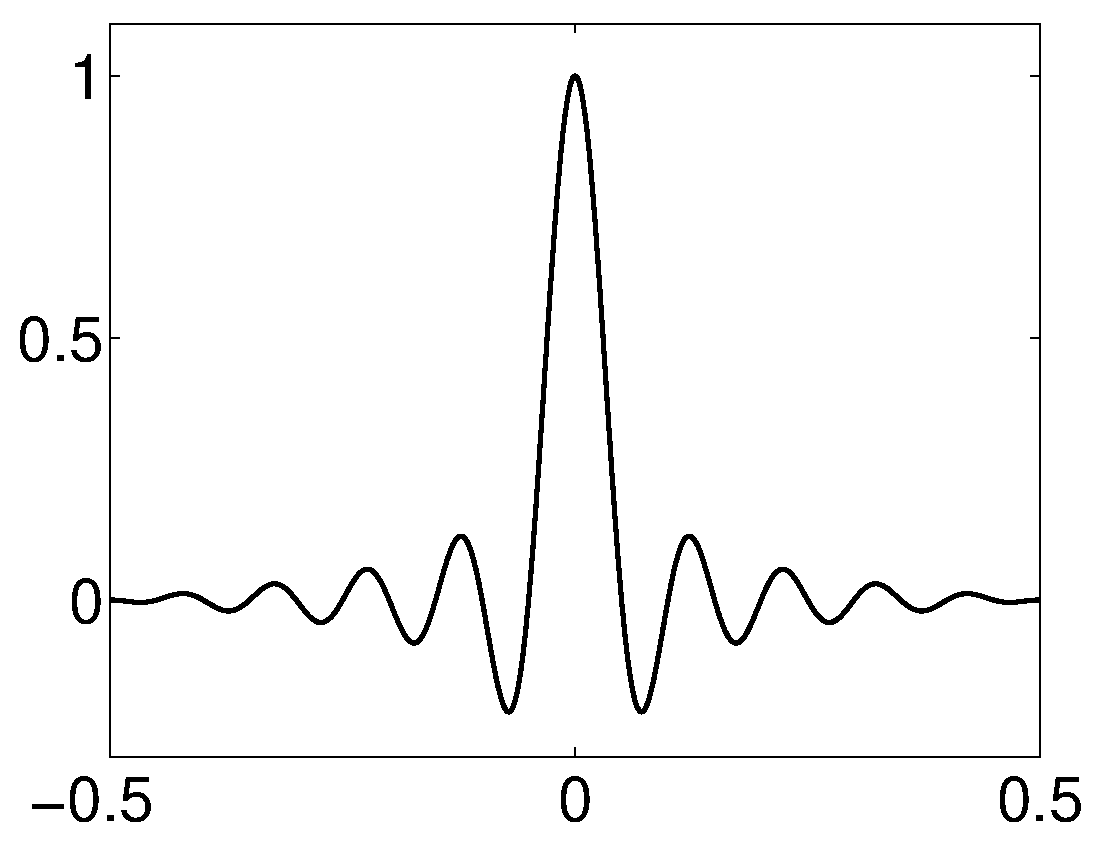
\includegraphics[width=4cm]{images/polynomial_kernels1.eps} &
      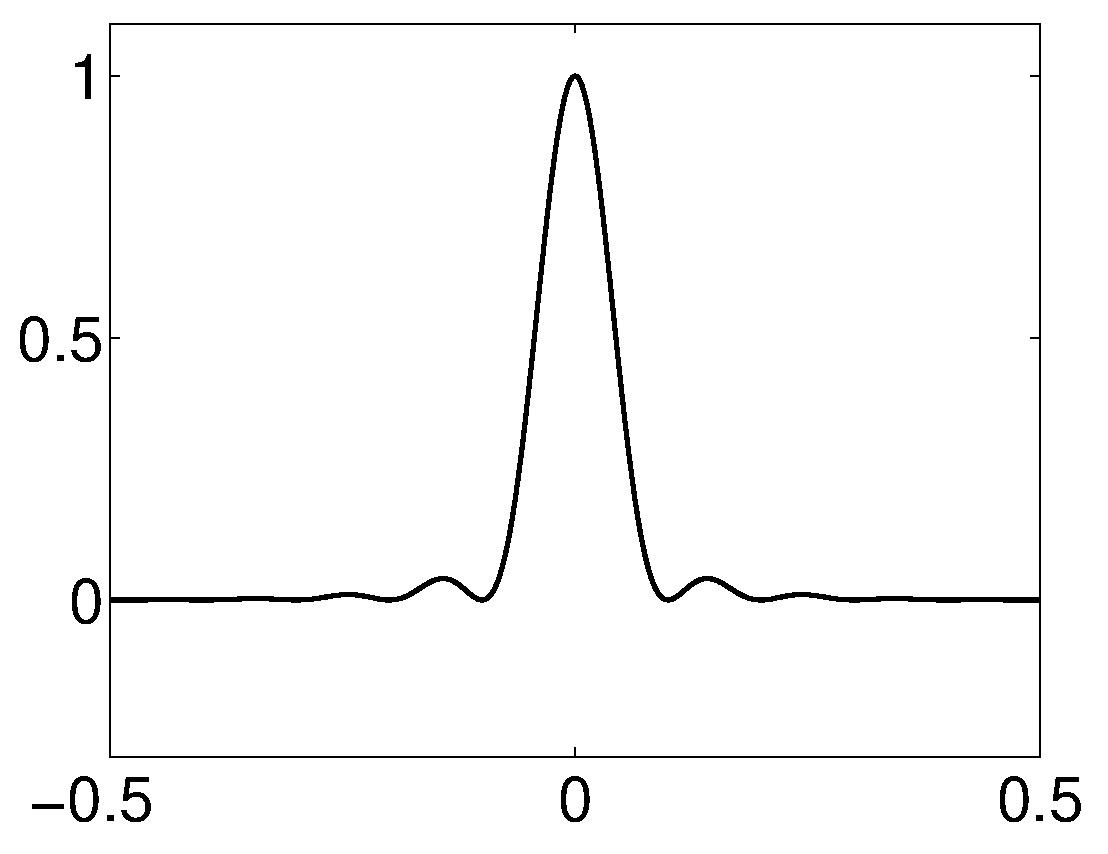
\includegraphics[width=4cm]{images/polynomial_kernels2.eps} &
      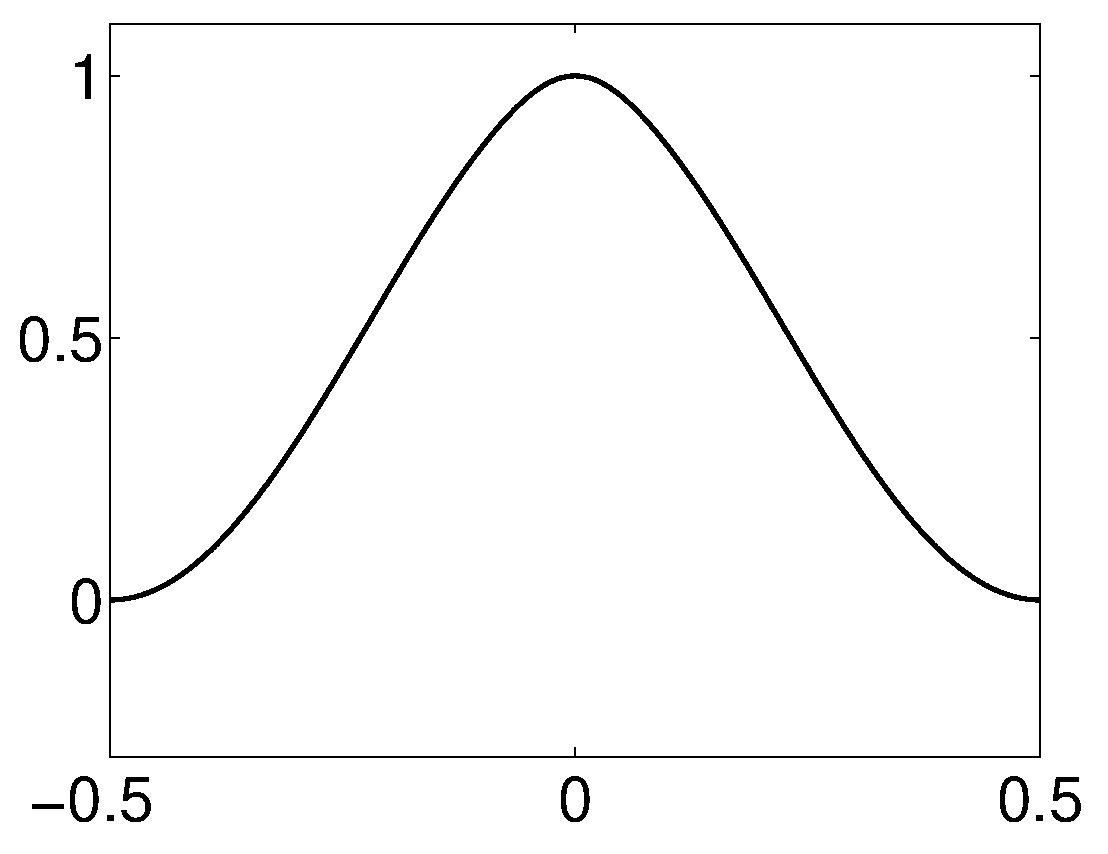
\includegraphics[width=4cm]{images/polynomial_kernels4.eps}
    \end{tabular}
  \end{center}
  \caption{From left to right: Real part of Dirichlet kernel $D_{20}$, the
    Fejer kernel $B_{2,20}$, and the Sobolev kernel
    $S_{1,2,10^{-4},20}$. \label{Fig:polykerne}}
\end{figure}

\begin{figure}[ht]
  \begin{center}
    \begin{tabular}{ccc}
      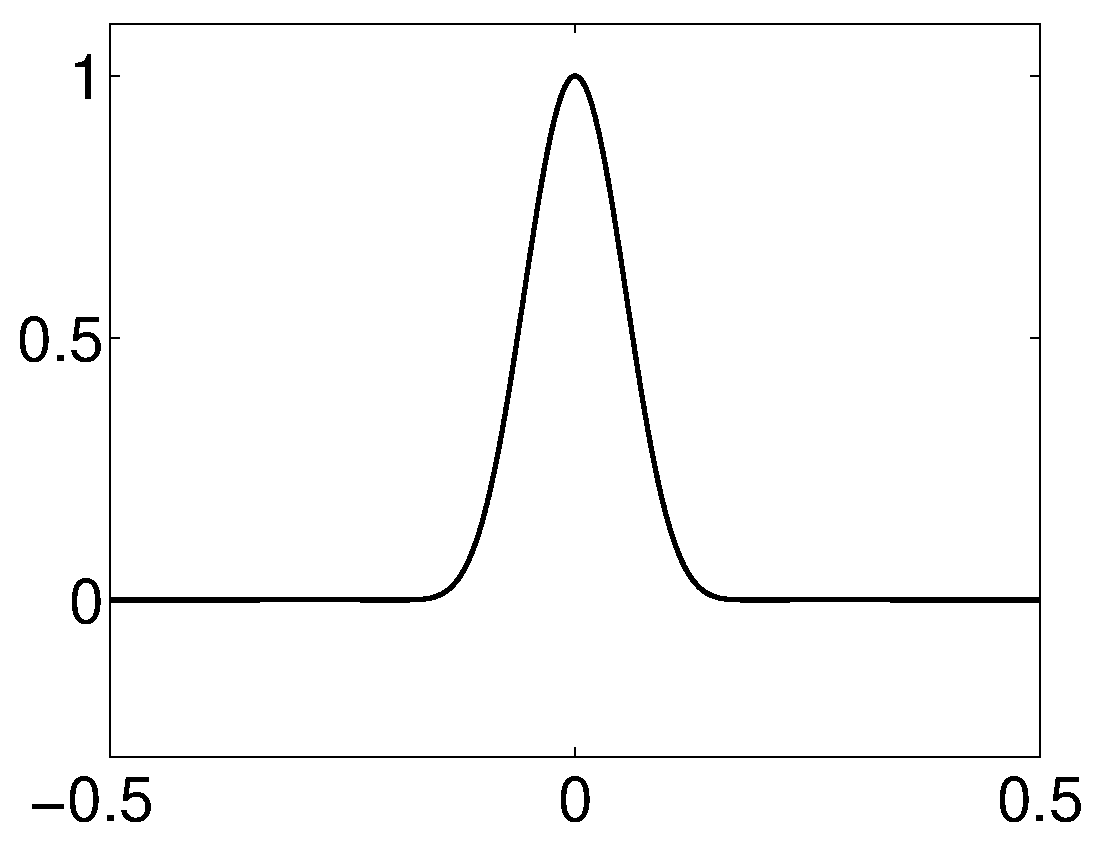
\includegraphics[width=4cm]{images/polynomial_kernels3.eps} &
      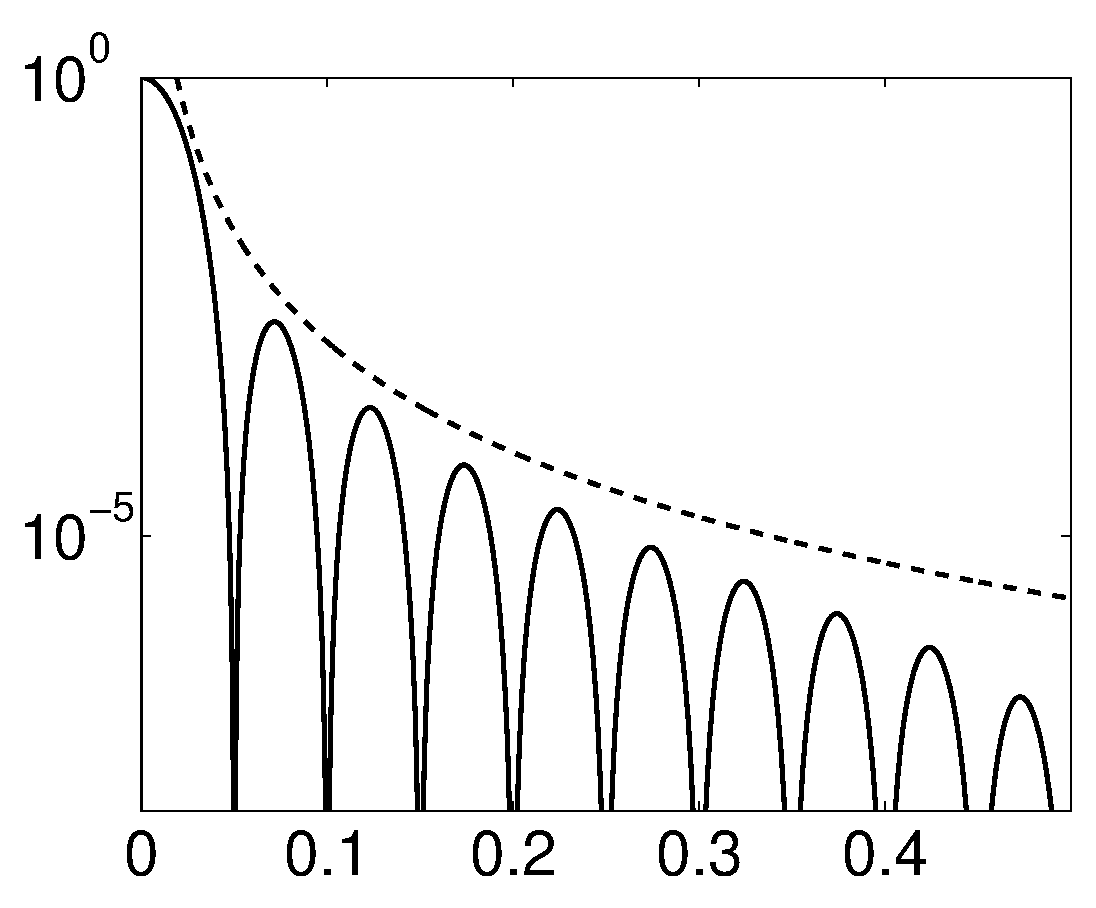
\includegraphics[width=4cm]{images/polynomial_kernels5.eps} &
      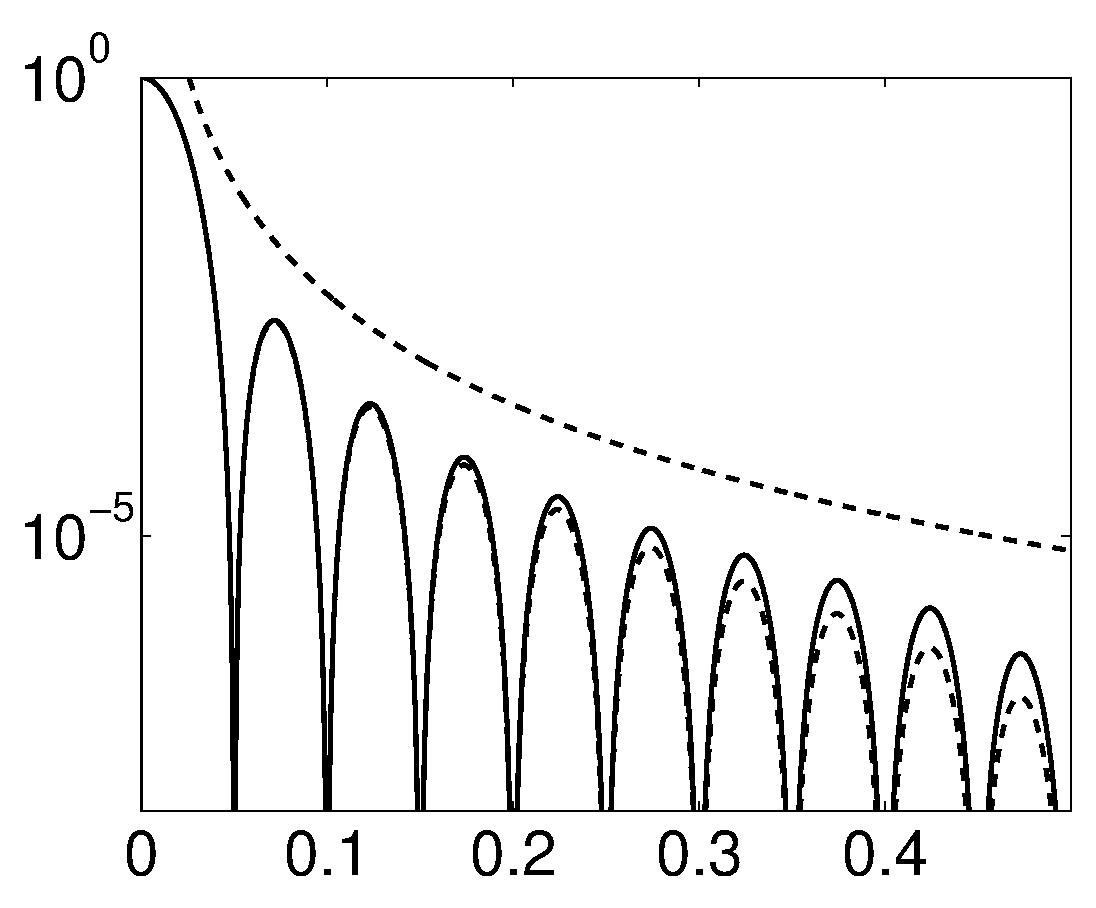
\includegraphics[width=4cm]{images/polynomial_kernels6.eps}
    \end{tabular}
  \end{center}
  \caption{Left: Real part of the B-Spline kernel $B_{4,20}$.
    Middle: Log plot of the modulus $|B_{4,80}|$ (solid) and the estimate by
    Corollary \ref{cor:spline} (dashed).
    Right: Log plot of the modulus Jackson kernel $|J_{4,78}|$, its decay
    estimate, cf. Example \ref{ex:kernels}, and the slightly better localised
    B-Spline kernel $|B_{4,80}|$ (dashed). \label{Fig:polykerne2}}
\end{figure}

We complete this section by an extension of our result to the multivariate
case $d>1$.
Indeed, tensor products of the kernels constructed in Theorem
\ref{theorem:T1_smooth} yield also localised multivariate kernels as shown in
the following corollary.

\begin{Corollary}\label{cor:tensorproduct}
  Let the univariate kernel $\tilde K_N$, cf. Definition
  \ref{def:kernel}, fulfil for some $\beta\in\N$, some constant $C_{\beta}>1$,
  and $x\in\left[-\frac{1}{2}, \frac{1}{2}\right]\setminus\left\{0\right\}$
  the decay condition $|\tilde K_N(x)| \le C_{\beta} |Nx|^{-\beta}$, then its
  tensor product kernel $K_N(\zb x)=\prod\limits_{t=0}^{d-1} \tilde K_N(x_t)$
  fulfils
  \begin{equation*}
    \left|K_N\left(\zb x\right)\right| \le \frac{C_{\beta}}
    {N^{\beta}\|\zb x\|_{\infty}^{\beta}}
  \end{equation*}
  for $\zb x\in\left[-\frac{1}{2}, \frac{1}{2}\right]^d\setminus\left\{\zb
  0\right\}$, with the same order of decay $\beta$ and constant $C_{\beta}$.
\end{Corollary}

Proof.
The assertion follows simply from the estimate $|K_N(\zb x)| \le |\tilde
K_N(\|\zb x\|_{\infty})|$. \Box

%-----------------------------------------------------------------------------
\section{Stability of the interpolation problem}
%-----------------------------------------------------------------------------
The trigonometric interpolation problem has a unique solution for $d=1$ and
almost sure a unique solution for $d>1$ whenever $N\ge q^{-1}$, since this
implies $N\ge M^{\frac{1}{d}}$ and all nodes are pairwise distinct.
However, the problem might be ill-posed and there is no way computing a
solution in a stable way.

In this section, we prove stability results for the trigonometric
interpolation problem at $q$-separated nodes in the univariate case,
cf. Theorem \ref{theorem:T1allgemein} and the multivariate case, cf. Theorem
\ref{theorem:Tdallgemein}.
Basically, a localised kernel $K_N$ yields a diagonal dominated kernel matrix
$\zb K_N$ for $q$-separated nodes.
Furthermore, we prove stability results for a slightly generalised
interpolation problem at equispaced nodes and subsets of equispaced nodes,
cf. Theorem \ref{theorem:eq}.
These results are applied to particular kernels from Section
\ref{sect:kernels} in Corollary \ref{cor:eq} and Corollary \ref{cor:qsep}.

\subsection*{The univariate setting}
The following theorem gives estimates for the extremal eigenvalues of the
matrix $\zb K_N$ under reasonable assumptions on the kernel $K_N$.
\begin{Theorem} \label{theorem:T1allgemein}
  Let $N \in 2\mathbb{N}$ be given and let the kernel $K_N$, cf. Definition
  \ref{def:kernel}, fulfil for some $\beta> 1$ and
  $x\in\left[-\frac{1}{2},\frac{1}{2}\right]\setminus \left\{0\right\}$ 
  the localisation property
  \begin{equation*}
    \left| K_N\left(x\right)\right| \le \frac{C_{\beta}}{ N^{\beta}
      |x|^{\beta}}\,.
  \end{equation*}
  Furthermore, let a sampling set ${\cal X}$ contain arbitrary nodes with
  separation distance $q>0$.
  Then, the extremal eigenvalues of the matrix $\zb K_N$ are bounded by
  \begin{equation*}
    1 -  \frac{2\, \zeta\left(\beta\right) C_{\beta}}{N^{\beta} q^{\beta}}
    \le \lambda \le 1 \le \Lambda \le
    1 + \frac{2\, \zeta\left(\beta\right) C_{\beta}}{N^{\beta}  q^{\beta}}.
  \end{equation*}
\end{Theorem}

Proof.
Let $\lambda_{\star}$ be an arbitrary eigenvalue of $\zb K_N$ and $M$ denote
the number of nodes in $\cal X$.
Then, for some index $j\in\left\{0,\hdots,M-1\right\}$ Gershgorin's circle theorem
yields
\begin{equation*}
  \left|\lambda_{\star}-1\right|
  \le \sum\limits_{l=0; l\ne j}^{M-1}
  \left|K_N\left(x_j-x_l\right)\right| \, ,
\end{equation*}
where we use $K_N\left(0\right)=1$, cf. Definition \ref{def:kernel}.
Furthermore, by using that the separation distance of the sampling set is $q$,
and by the localisation of the kernel $K_N$, we obtain
\begin{eqnarray*}
  \left|\lambda_{\star}-1\right|
  &\le & \frac{C_{\beta}}{N^{\beta} }\sum\limits_{l=0; l\ne j}^{M-1}
  \frac{1}{\left| x_j-x_l\right|^\beta}
  \le  \frac{2 \, C_{\beta}}{N^{\beta} q^{\beta}}
  \sum\limits_{l=1}^{\left\lfloor M/2\right\rfloor} l^{-\beta}
    <   \frac{2\,\zeta(\beta) C_{\beta}}{N^{\beta} q^{\beta}}.
\end{eqnarray*}
\Boxgl

Indeed, the kernels constructed in Theorem \ref{theorem:T1_smooth} yield well
conditioned matrices $\zb K_N$.
As an immediate consequence of Theorem \ref{theorem:T1allgemein} we state a
stability result for an equispaced grid disturbed by jitter.
\begin{Corollary}\label{cor:jitter}
  Let the assumptions of Theorem \ref{theorem:T1allgemein} hold true.
  Furthermore, let the sampling nodes be of the form
  $x_j=-\frac{1}{2}+\frac{j-\varepsilon_j}{M},\; j=0,\hdots,M-1,$ where
  $0\le\varepsilon_j \le \varepsilon < 1$.
  Then the eigenvalues of the matrix $\zb K_N$ are bounded by
  \begin{equation*}
    1-\frac{2\, \zeta\left(\beta\right) C_{\beta} M^{\beta}}{N^{\beta} \left(1-
        \varepsilon \right)^{\beta}} \le \lambda \le 1 \le \Lambda \le
    1+\frac{2\, \zeta\left(\beta\right) C_{\beta} M^{\beta}}{N^{\beta} \left(1-
        \varepsilon \right)^{\beta}}\,.
  \end{equation*}
\end{Corollary}

Proof. Since the separation distance is bounded by $q\ge M^{-1}
(1-\varepsilon)$ the result follows by Theorem \ref{theorem:T1allgemein}. \Box

\subsection*{The multivariate setting}
First, we show in Lemma \ref{lemma:Tda} how many $q$-separated nodes can be
placed in a certain distance to a reference node, see also Figure
\ref{fig:Td}.
A similar method is  used in \cite{NaSiWa98} for the $d$-sphere.

\begin{Definition}\label{def:part}
  For $d\in\N$ and a separation distance $q \le \frac{1}{2}$, we define the
  partitioning
  \begin{equation*}
    R_{q,m}:=
    \left\{\zb x \in \T^d:m q \le \dist\left(\zb x,\zb
    0\right)<\left(m+1\right)q\right\}
  \end{equation*}
  for $m=0,\hdots,\left\lfloor q^{-1}/2 \right\rfloor-1$ and
  \begin{equation*}
    R_{q,\left\lfloor q^{-1}/2 \right\rfloor}:=
    \left\{\zb x \in \T^d: \left\lfloor q^{-1}/2 \right\rfloor q \le
    \dist\left(\zb x,\zb 0\right)\le 1/2\right\}.
  \end{equation*}
  Its restriction to the sampling set ${\cal X}$ will be denoted by $R_{{\cal
      X},q,m}:=R_{q,m}\cap {\cal X}$.
\end{Definition}

\begin{figure}[ht!]
  \begin{center}
    \psset{unit=0.7cm}

%% q=1 unit

\begin{pspicture}(10,10)
 \psframe[linestyle=dashed](0,0)(10,10)
 \put(0.2,0.2){\framebox(9.6,9.6){}}
 \put(0.3,0.5){$R_{q,\left\lfloor q^{-1}/2 \right\rfloor}$}

 \put(1,1){\framebox(8,8){}}
 \put(1.1,1.3){$R_{q,\left\lfloor q^{-1}/2 \right\rfloor-1}$}
 \put(2,2){\framebox(6,6){}}

 \put(2.2,5.1){$\hdots$}
 \put(7.2,5.1){$\hdots$}

 \put(3,3){\framebox(4,4){}}
 \put(3.1,3.3){$R_{q,1}$}
 \put(4,4){\framebox(2,2){}}
 \put(4.1,4.3){$R_{q,0}$}

 \put(4.8,5){\line(1,0){0.4}}
 \put(5,4.8){\line(0,1){0.4}}
 \put(5.1,5.1){$\zb x_0$}

%\put(2,3){\makebox(3,7)[rb]{Dieser Text erscheint rechts unten in der Box.}}
\end{pspicture}

%%% Local Variables: 
%%% mode: latex
%%% TeX-master: "~/Nfft3/nfft/trunk/doc/paper/stability/stability"
%%% End: 

  \end{center}
  \caption{Partitioning of the torus $\mathbb{T}^2$ (solid) where the
      outermost 'ring' $R_{q,\left\lfloor q^{-1}/2 \right\rfloor}$ is enlarged
      (dashed) as in the proof of Lemma \ref{lemma:Tda}.\label{fig:Td}}
\end{figure}

\begin{Lemma} \label{lemma:Tda}
   Let $d\in \N$ and an $q$-separated sampling set ${\cal X}$ with $q \le
   \frac{1}{2}$ be given.
   Then, each of the sets $R_{{\cal X},q,m}$ has bounded cardinality
   \begin{equation*}
     \left|R_{{\cal X},q,m}\right|\le 2^d\left(2^d-1\right) m^{d-1},
     \qquad m=1,\hdots,\left\lfloor q^{-1}/2 \right\rfloor.
   \end{equation*}
\end{Lemma}
Proof. The assertion follows from
\begin{equation*}
  \left|R_{{\cal X},q,m}\right| \le \frac{1}{q^d}
  \int\limits_{R_{q,m} } \d \zb x \le
  2^d\left(\left(m+1\right)^d-m^d\right)
  =2^d\sum_{t=1}^d {d\choose t} m^{d-t}
  \le 2^d m^{d-1} \sum_{t=1}^d {d\choose t}.
\end{equation*}
\Boxgl

Using localised kernels in conjunction with a separated sampling set and Lemma
\ref{lemma:Tda}, we state the following theorem on the stability of the
interpolation problem.

\begin{Theorem} \label{theorem:Tdallgemein}
  Let $d\in\N$, $N \in 2\mathbb{N}$ be given and let the kernel $K_N$,
  cf. Definition \ref{def:kernel}, fulfil for some $\beta> d$ and
  $\zb x\in\left[-\frac{1}{2},\frac{1}{2}\right]^d\setminus\left\{\zb
  0\right\}$ the localisation property
  \begin{equation*}
    \left|K_N\left(\zb x\right)\right| \le \frac{C_{\beta}}
    {N^{\beta}\|\zb x\|_{\infty}^{\beta}}\,.
  \end{equation*}
  Furthermore, let a sampling set ${\cal X}$ contain arbitrary nodes with
  separation distance $0<q\le \frac{1}{2}$.
  Then, the extremal eigenvalues of the matrix $\zb K_N$ are bounded by
  \begin{equation*}
    1 - \frac{2^d\left(2^d-1\right) \zeta\left(\beta-d+1\right)
    C_{\beta}}{N^{\beta} q^{\beta}} \le \lambda \le 1 \le \Lambda \le
    1 + \frac{2^d\left(2^d-1\right) \zeta\left(\beta-d+1\right)
    C_{\beta}}{N^{\beta} q^{\beta}}.
  \end{equation*}
\end{Theorem}

Proof. 
Let $\lambda_{\star}$ be an arbitrary eigenvalue of $\zb K_N$.
Without loss of generality, let the diagonal element of the matrix $\zb K_N$
used in Gershgorin's circle theorem correspond to $\zb x_0=\zb 0$.
Then we conclude by $K_N(\zb 0)=1$, cf. Definition \ref{def:kernel}, that
\begin{eqnarray*}
  \left|\lambda_{\star}-1\right| &\le& \sum\limits_{l=1}^{M-1} \left|
    K_N\left(\zb 0-\zb x_l\right)\right|.
\end{eqnarray*}
Using $q\le\frac{1}{2}$, the partition from Definition \ref{def:part}, Lemma
\ref{lemma:Tda}, and the localisation of the kernel $K_N$, we get
 \begin{eqnarray*}
 \left|\lambda_{\star}-1\right|
     &\le&\sum\limits_{m=1}^{\left\lfloor q^{-1}/2 \right\rfloor}
     \sum\limits_{\zb x_l \in R_{{\cal X},q,m}} 
     \left|K_N\left(-\zb x_l\right)\right|\\
     &\le& \frac{2^d\left(2^d-1\right) C_{\beta}}{N^{\beta}}
     \sum\limits_{m=1}^{\left\lfloor q^{-1}/2 \right\rfloor} m^{d-1}
     \max\limits_{\zb x \in R_{q,m}} \|\zb x\|_{\infty}^{-\beta}\\ 
     &\le& \frac{2^d\left(2^d-1\right) \zeta\left(\beta-d+1\right)
     C_{\beta}}{N^{\beta} q^{\beta}}.
   \end{eqnarray*}
\Boxgl

Particularly, this result includes Theorem \ref{theorem:T1allgemein} if we set
$d=1$. 

\subsection*{Equispaced nodes} \label{sect:eq}
In the case of equispaced nodes we employ the fact that the matrix $\zb K_N$
is circulant.
We present a slightly generalised result in the following Theorem
\ref{theorem:eq}.

\begin{Definition}  \label{def:l1kernel}
  We define for $d,n\in\N$ and weights $\hat w_{\zb k} \in \R,\; \zb k \in
  \Z^d$ with $\sum_{\zb k\in \Z^d}|\hat w_{\zb k}| < \infty$, the kernel
  \begin{equation*}
    K \left(\zb x\right):=\sum\limits_{\zb k \in \Z^d} \hat w_{\zb k}
    \eip{\zb k \zb x}
  \end{equation*}
  and by evaluating at the equispaced sampling nodes $\zb x_{\zb j} :=
  n^{-1}(j_0,\hdots,j_{d-1})^{\top}$, $\zb j\in I_n$, the kernel matrix
  \begin{equation*}
    \zb K: = \left(K (\zb x_{\zb j}-\zb x_{\zb l}) \right)_{\zb j,\zb l \in
    I_n} \in \C^{n^d\times n^d}.
  \end{equation*}
\end{Definition}

\begin{Theorem}\label{theorem:eq}
  Let $d\in\N$, the sampling set $\cal X$ consist of $M=n^d$, $n\in\N$,
  equispaced nodes, and the kernel $K$ be given by Definition
  \ref{def:l1kernel}, then:
  \begin{enumerate}
  \item The kernel matrix $\zb K$ has the
    eigenvalues
    \begin{equation*}
      \lambda_{\zb j}\left(\zb K\right)
      = n^d\sum\limits_{\zb r\in \Z^d} \hat w_{\zb j+n\zb r}\, .
    \end{equation*}
  \item For tensor product weights $\hat w_{\zb k}=\prod_{t=0}^{d-1} \hat
    w_{k_t}$, the eigenvalues possess the same property $\lambda_{\zb
    j}=\prod_{t=0}^{d-1} \lambda_{j_t}$ where $\lambda_{j_t}$ denotes the
    $j_t$th eigenvalue of the univariate interpolation matrix constructed from
    the damping factors $(\hat w_{k_t})_{{k_t} \in \Z}$ and the nodes
    $x_j=\frac{j}{n}$, $j=-\frac{n}{2},\hdots,\frac{n}{2}-1$.
  \item The extremal eigenvalues remain bounded by the extremal eigenvalues of
    $\zb K$ if one removes nodes from $\cal X$.
  \end{enumerate}
\end{Theorem}

Proof.
\begin{enumerate}
\item The multilevel circulant matrix $\zb K$ is diagonalised by the Fourier
  matrix $\zb F_n=(\eip{\zb k\zb x_{\zb j}})_{\zb j,\zb k\in I_n}$.
  See also \cite[Cor. 3.10, Thm. 3.11]{NaSiWa98} for the univariate case.
\item This property is due to the Kronecker product structure of the matrix
  $\zb K$ in the case of tensor product kernels.
\item The last assertion follows from the fact that removing a node is nothing
  else than removing its corresponding row and column in $\zb K$ and from the
  interlacing property for eigenvalues, see \cite[pp. 185]{HoJo}.
\end{enumerate}
\Box

\subsection*{Applications} \label{sect:appl}
We apply the result of the Theorems \ref{theorem:T1allgemein},
\ref{theorem:Tdallgemein}, and \ref{theorem:eq} to the B-Spline kernels from
Definition \ref{def:spline} and the kernels given in Example
\ref{ex:kernels}.
\begin{Corollary}  \label{cor:eq}
  Let the dimension $d\in\N$, a sampling set $\cal X$ with $M\ge 2$ equispaced
  nodes, and a polynomial degree $N\in 2\mathbb{N}$ with
  $N>q^{-1}=M^{\frac{1}{d}}$ be given.
  Then, for the Dirichlet kernel, cf. Example \ref{ex:kernels} i),
  and its tensor product version for $d>1$, the following estimates for the
  extremal eigenvalues $\lambda,\Lambda$ of the kernel matrix $\zb K_N$ hold
  true
  \begin{equation*}
    \left(\frac{1}{Nq}\left\lfloor Nq \right\rfloor\right)^d
    = \lambda \le 1 \le \Lambda =
    \left(\frac{1}{Nq}\left\lceil{Nq}\right\rceil\right)^d.
  \end{equation*}
  Furthermore, for the Fejer kernel we have
  \begin{equation*}
    \left(1- \frac{1}{ N^2q^{2}}\right)^d
    \le \lambda \le 1 \le \Lambda \le
    \left(1+ \frac{1}{ N^2q^{2}}\right)^d
  \end{equation*}
  where equality holds for the outmost inequalities if
  $N=\left(2\sigma+1\right)q^{-1},\,\sigma\in\mathbb{N}$.
  In particular, the kernel matrix $K_N$ is non singular.
\end{Corollary}

Proof. Throughout this proof, let $n=q^{-1}$ and the damping factors be
extended by $\hat w_{\zb k}=0$ for $\zb k \notin \indexset$.
We apply for $d=1$ Theorem \ref{theorem:eq} i) to the weights
$\hat w_k= \frac{1}{N}$, $k \in I_N$, of the Dirichlet kernel for $N\in 2\N$
and to the weights $\hat w_k= \frac{2}{N}(1-\frac{|2k+1|}{N})$, $k \in I_N$,
of the Fejer kernel, if $N=\left(2\sigma+1\right)q^{-1},\,\sigma\in
\mathbb{N}$, respectively.

The assertion is little more delicate for the univariate Fejer kernel and
$N\neq\left(2\sigma+1\right)q^{-1}$.
We use the representation
\begin{equation*}
  \left|B_{2,N}\left(x\right)\right| = \frac{4}{N^2}
  \sum\limits_{r=0}^{\frac{N}{2}-1} \sum\limits_{k=-r}^{r} \eip{kx}.
\end{equation*}
Now, let $\lambda_{\star}$ be an arbitrary eigenvalue of the kernel matrix
$K_N$, then Gershgorin's circle theorem yields
\begin{equation*}
  \left|\lambda_{\star}-1\right|
  \le \sum_{l=1}^{n-1}\left|B_{2,N}\left(\frac{l}{n}\right)\right|
%  &=&\frac{4n}{N^2} \left(\sum\limits_{r=0}^{\frac{N}{2}-1}
%    \sum\limits_{k=-r}^{r} \delta_{k,0}^{(n)}\right) - 1\\
   = \frac{4n}{N^2} \sum\limits_{r=0}^{\frac{N}{2}-1}
   \left(2\left\lfloor \frac{r}{n} \right\rfloor+1\right) - 1.
\end{equation*}
Since for $Q:=\left\lfloor\frac{N-2}{2n}\right\rfloor$ and $R:=\frac{N}{2}-1-nQ$ the identity
\begin{equation*}
  \sum\limits_{r=0}^{\frac{N}{2}-1}\left\lfloor \frac{r}{n} \right\rfloor
  =\sum\limits_{s=0}^{Q-1}\;\sum\limits_{r=sn}^{\left(s+1\right)n-1} s + \sum_{r=nQ}^{nQ+R} Q
  =\frac{\left(N-n\right)^2 - \left(2\left(R+1\right)-n\right)^2}{8n}
\end{equation*}
holds, we proceed
\begin{eqnarray*}
  \frac{4n}{N^2} \sum\limits_{r=0}^{\frac{N}{2}-1}
  \left(2\left\lfloor \frac{r}{n} \right\rfloor+1\right) - 1
  &= &\frac{4n}{N^2} \left(2 \frac{\left(n-N\right)^2 - \left(2\left(R+1\right)-n\right)^2}{8n} + \frac{N}{2}\right) - 1\\
  &= &\frac{n^2}{N^2}-\left(\frac{2\left(R+1\right)-n}{N}\right)^2\\
  &\le & \frac{n^2}{N^2}.
\end{eqnarray*}

The case $d>1$ is due to Theorem \ref{theorem:eq} ii).
\Box

Note that the above inequalities remain true if an arbitrary subset of the
nodes is removed, cf. Theorem \ref{theorem:eq} iii).
Next, we give estimates for the stability of interpolation problem at
arbitrary nodes.
\begin{Corollary}  \label{cor:qsep}
  Let the dimension $d\in\N$ and an arbitrary sampling set $\cal X$ with
  separation distance $q\le\frac{1}{2}$ be given, then the eigenvalues of the
  kernel matrix are bounded away from zero as follows.
  \begin{enumerate}
  \item For the Dirichlet kernel, $d=1$, $N\in 2\N$, and
    $N>\left(1+\left|\log\left(2q\right)\right|\right)q^{-1}$ holds 
    \begin{equation*}
      1- \left(1+\left|\log\left(2q\right)\right|\right)\frac{1}{Nq}
      \le \lambda \le 1 \le \Lambda \le
      1+ \left(1+\left|\log\left(2q\right)\right|\right)\frac{1}{Nq}.
    \end{equation*}
  \item For the B-Spline kernel of order $\beta=d+1$, $N\in 2\N$, $N\ge
    2\beta$, and $N>2dq^{-1}$ holds
    \begin{equation*}
      1- \left(\frac{2d}{Nq}\right)^{d+1}
      \le \lambda \le 1 \le \Lambda \le
      1+ \left(\frac{2d}{Nq}\right)^{d+1}\,,
    \end{equation*}
    where we simplified the involved constant.
  \item For the Jackson kernel of order $\beta=2\lceil\frac{d+1}{2}\rceil$,
    $N\in 2\N$, and $N>2.1 d q^{-1}$ holds
    \begin{equation*}
      1- \left(\frac{2.1d}{Nq}\right)^{d+1}
      \le \lambda \le 1 \le \Lambda \le
      1+ \left(\frac{2.1d}{Nq}\right)^{d+1}\,,
    \end{equation*}
    where we simplified the involved constant.
  \end{enumerate}
\end{Corollary}

Proof. We apply Theorem \ref{theorem:Tdallgemein} for ii) and iii) where we
 use the estimates for $C_{\beta}$ given in Corollary \ref{cor:spline} and
 Example \ref{ex:kernels} ii).
 Assertion i) follows along the same lines, i.e., we use the decay as given in
 Example \ref{ex:kernels} i) and only change the last step of Theorem
 \ref{theorem:T1allgemein} where we use $M\le q^{-1}$ and
 \begin{equation*}
   \sum\limits_{l=1}^{\left\lfloor M/2\right\rfloor} l^{-1} \le 1+\ln
   \frac{M}{2}.
 \end{equation*}
\Boxgl

Thus, we have shown that the optimal trigonometric interpolation problem at
$q$-separated nodes in $d$ dimensions is well conditioned for a polynomial
degree $N \ge 2 d q^{-1}$.
If we assume further the uniformity condition $q=c M^{-\frac{1}{d}}$ for a
sampling set of cardinality $M$, then the total arithmetical complexity for
solving \eqref{eq:optInterp} up to a prescribed error is of order ${\cal O}(M
\log M)$.
Note however, that the condition $N> 2 d q^{-1}$ is not optimal for high
dimensional problems.
As pointed out in \cite{BaGr04} for the approximation problem \eqref{eq:ap},
it is an open problem to improve these estimates.

%-----------------------------------------------------------------------------
\section{Numerical results}
%-----------------------------------------------------------------------------
In this section, we exemplify our findings on the stability of the optimal
interpolation problem \eqref{eq:optInterp} and its iterative solution by
Algorithm \ref{algo:CGNE}.

The estimates for the condition number of the kernel matrix $\zb K_N$ for
equispaced nodes, cf. Corollary \ref{cor:eq}, are shown in Figure
\ref{Fig:cond_eq_jitter} (left).
For $N=\sigma q^{-1}$ and the Dirichlet kernel $D_N$ the matrix $\zb K_N$ is
just the identity.
However, using the better localised Fejer kernel $B_{2,N}$ improves the
condition number already for $N>\sqrt{3}q^{-1}$ when $N\ne\sigma q^{-1}$.

We present the effect on the stability of the interpolation problem when the
equispaced nodes are perturbed by jitter error, cf. Corollary
\ref{cor:jitter}, in Figure \ref{Fig:cond_eq_jitter} (right).
We choose different sampling sets of size $M=1,\hdots,100$ with equispaced
nodes disturbed by $10\%$ jitter error and evaluate the maximum condition
number over $100$ reruns for the Dirichlet kernel $D_{6M}$ and the Fejer
kernel $B_{2,6M}$, respectively.
The Fejer kernel produces a lower condition number which is also validated by
the shown upper bound.

\begin{figure}[ht!]
  \begin{center}
    \begin{tabular}{cc}
      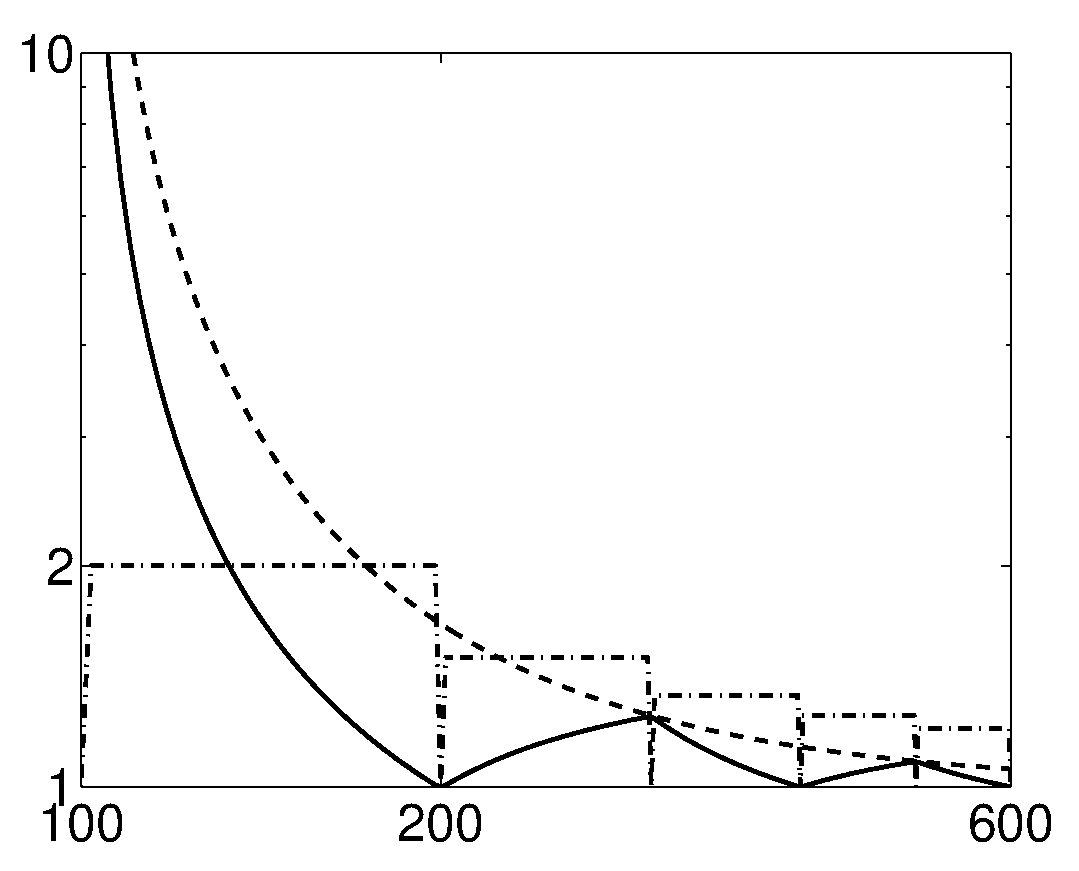
\includegraphics[width=6cm]{images/equidist_example1.eps}
      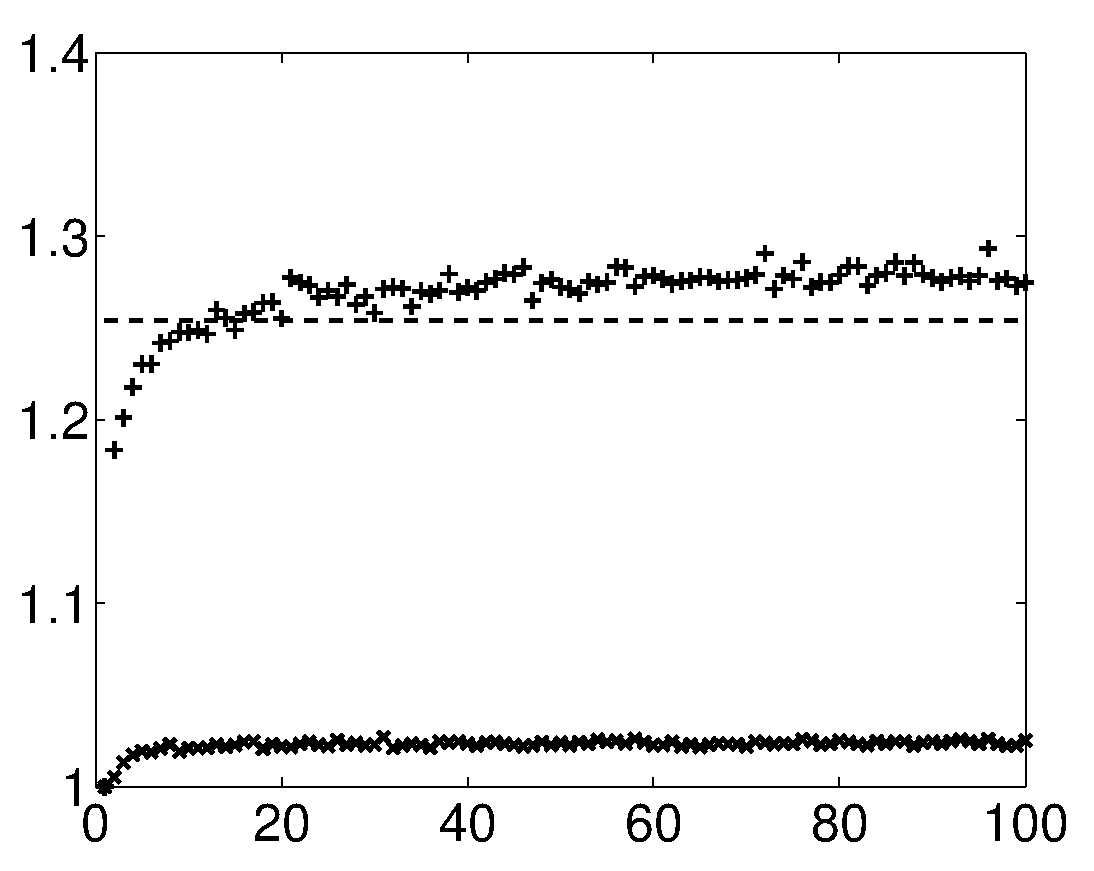
\includegraphics[width=6cm]{images/test_cond1.eps}
    \end{tabular}
  \end{center}
  \caption{Condition number of the kernel matrix $\zb K_N$.
    Left: Condition number with respect to polynomial degree
    $N=100,\hdots,600$, no weights, i.e., Dirichlet kernel (dash-dot); weight
    function $g_2$, i.e., Fejer kernel (solid), and the estimate of Corollary
    \ref{cor:eq}; here, the number of equispaced nodes is $M=100$.
    Right: Condition number with respect to the number of nodes
    $M=1,\hdots,100$, the nodes are equispaced perturbed by
    $\varepsilon_{\text{rel.}}=0.1$ jitter error, the polynomial degree is 
    $N=6M$;
    no weights, i.e., Dirichlet kernel ($\,+\,$);
    weight function $g_2$, i.e., Fejer kernel (${}\times{}$), and its estimate
    by Corollary \ref{cor:jitter} (dashed).\label{Fig:cond_eq_jitter}}
\end{figure}

Furthermore, we apply Algorithm \ref{algo:CGNE} using the NFFT software
package \cite{kupo02C} to reconstruct a univariate signal from randomly
scattered data in Figure \ref{fig:error_decay}, whereas Figure
\ref{Fig:glacier} shows the reconstruction of a bivariate signal from a
glacier data set \cite{Franke.Daten}. 
The main tool in our iterative algorithms is the NFFT, i.e., the fast matrix
times vector multiplication with $\zb A$ and $\zb A^{\adj}$, respectively.
Details concerning NFFT algorithms can be found for example in \cite{postta01}
and a software package can be found in \cite{kupo02C}.

The reconstruction of the randomly sampled univariate signal shows the decay
rates of our iterative scheme.
The sampling set consists of $M=100$ nodes separated by $q=4\times 10^{-3}$ and we
reconstruct with a polynomial degree $N=1000$ and the Dirichlet-, Fejer-,
B-Spline-, and Sobolev kernel.
All schemes converge within $15$ iteration where this is justified only for
the Fejer- and the B-Spline kernel.

\begin{figure}[ht]
  \begin{center}
    \begin{tabular}{cc}
      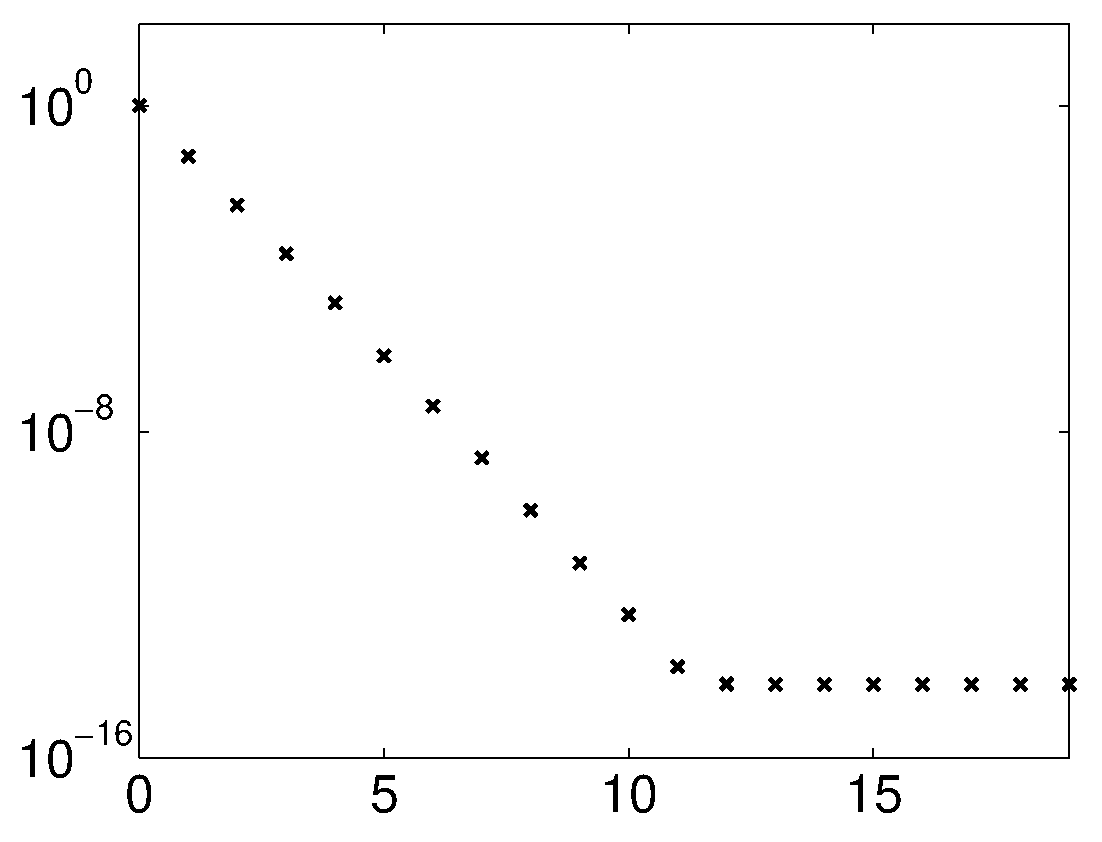
\includegraphics[width=6cm]{images/error_decay_4_0.eps} &
      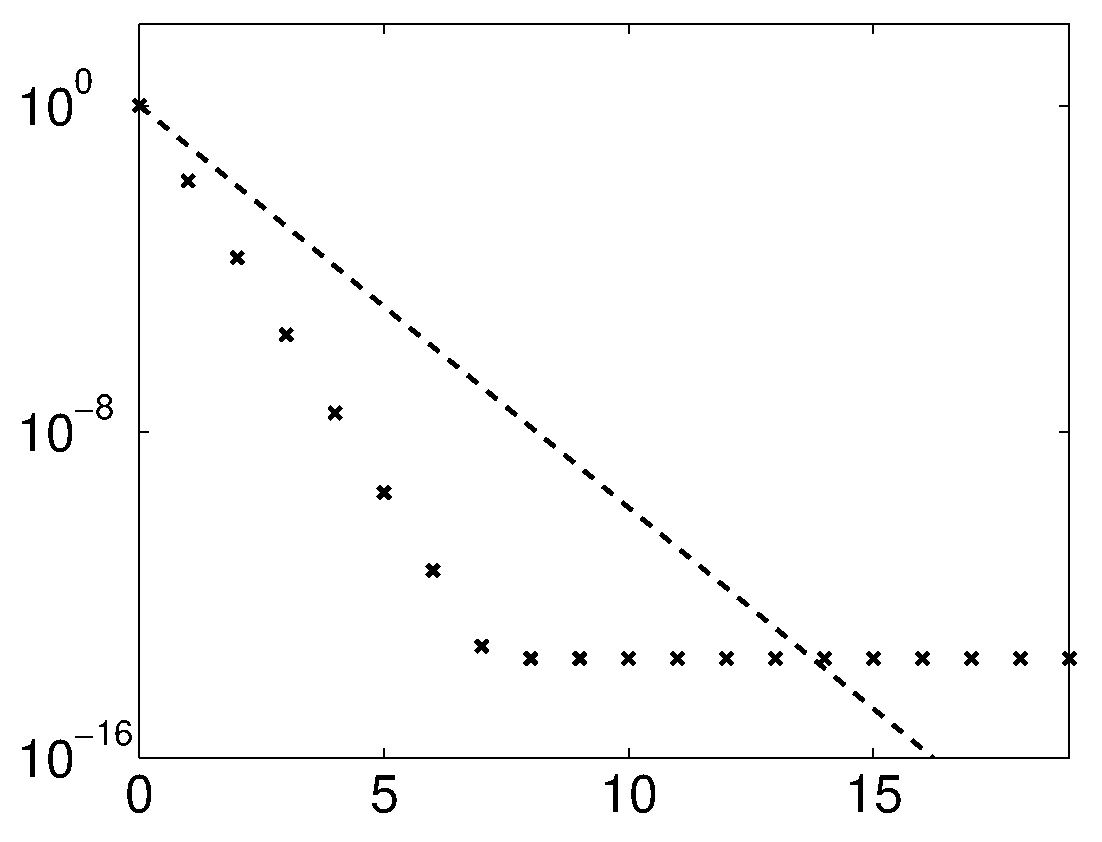
\includegraphics[width=6cm]{images/error_decay_4_1.eps} \\
      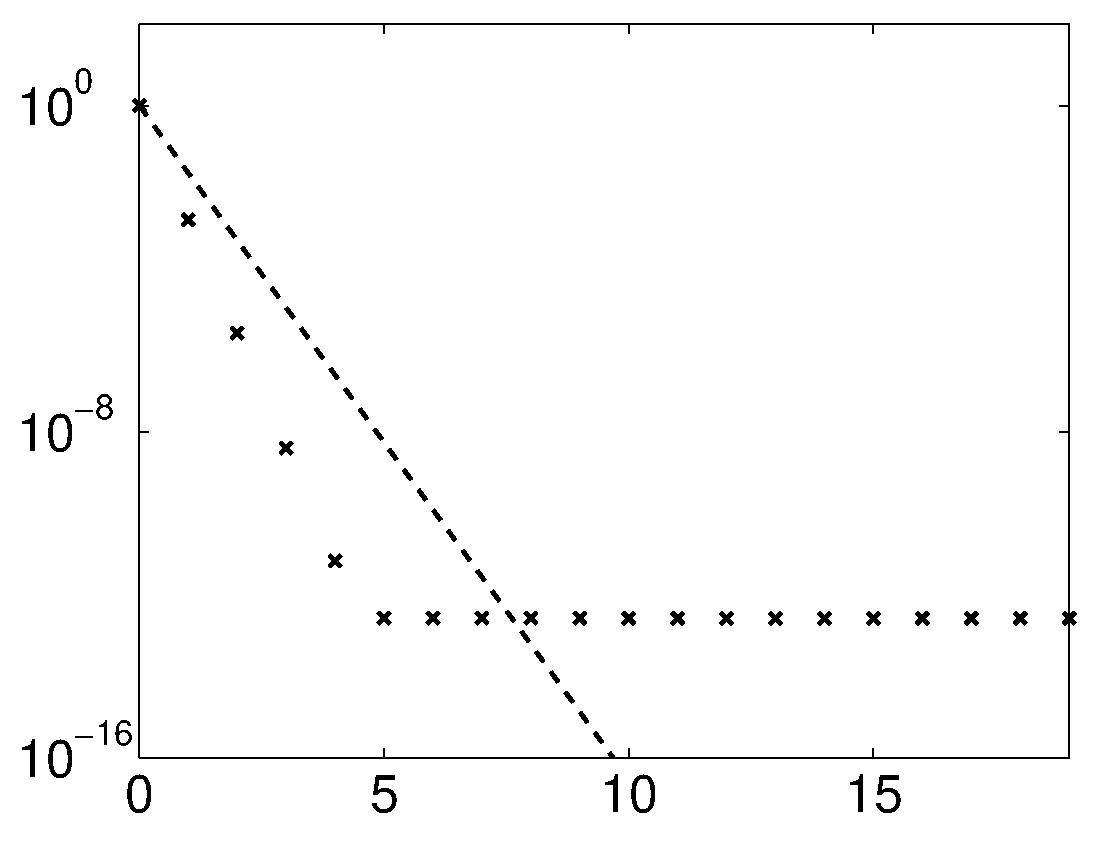
\includegraphics[width=6cm]{images/error_decay_4_2.eps} &
      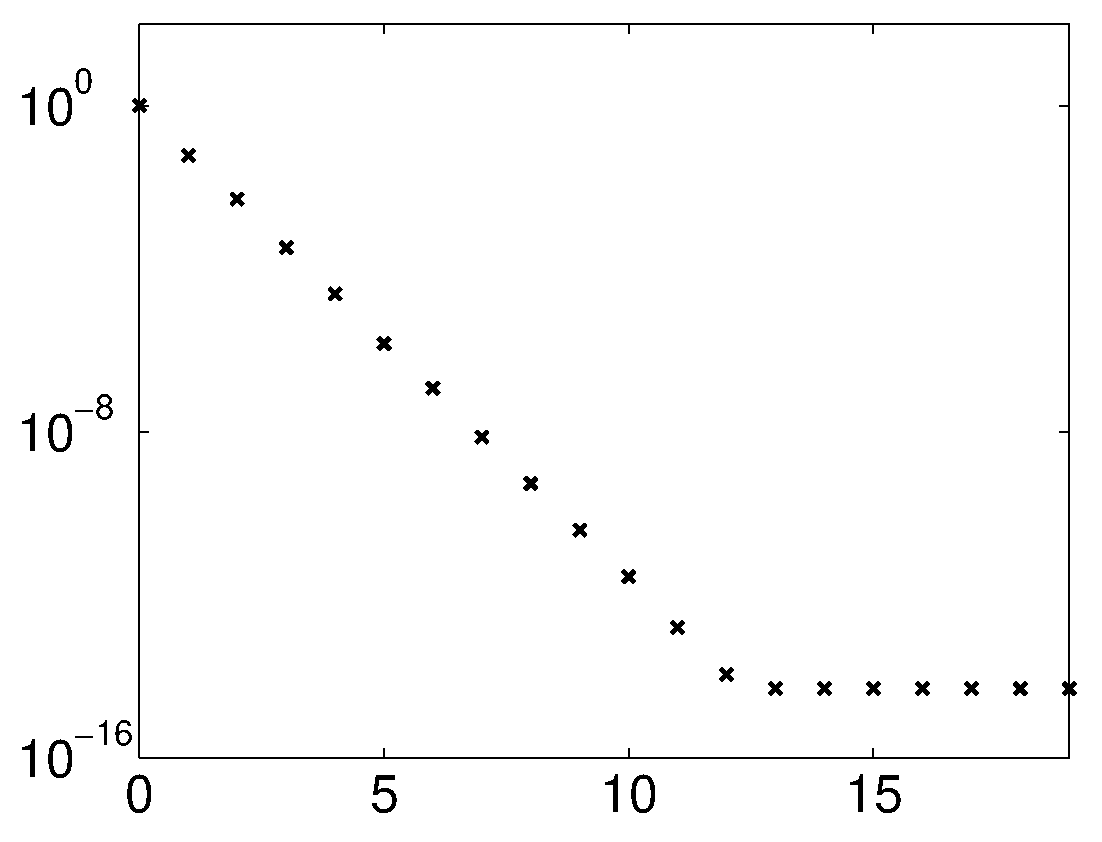
\includegraphics[width=6cm]{images/error_decay_4_3.eps} 
    \end{tabular}
  \end{center}
  \caption{Native error $\|\zb {\hat f}_l-\zb {\hat W} \zb A^{\adj} \zb
    K_N^{-1} \zb y\|_{\zb {\hat W}^{-1}}$ for the univariate interpolation
    problem with respect to the current iteration $l$.
    The number of samples is $M=100$, the number of computed Fourier
    coefficients is $N=1000$, and the separation distance of the nodes is
    $q=4\times 10^{-3}$.
    Top left: no weights, i.e., Dirichlet kernel;
    Top right: weight function $g_2$, i.e., Fejer kernel, predicted decay rate
    (dashed);
    Bottom left: weight function $g_4$, i.e., B-Spline kernel, predicted decay rate
    (dashed);
    Bottom right: weight function $g_{1,2,10^{-2}}$, i.e., Sobolev kernel.
    \label{fig:error_decay}}
\end{figure}


The last example shows a typical test case for radial basis function methods.
We reconstruct from a data set of $M=8345$ samples on level curves of a
glacier a total number of $2^{16} \approx 8 M$ Fourier coefficients.
Note however, that the sampling set is highly nonuniform in the sense that the
separation distance is very small compared to the mesh norm.
The assumptions of Theorem \ref{theorem:Tdallgemein} are not fulfilled,
nevertheless, the proposed method yields a very good approximation to the
given data after $40$ iterations.

\begin{figure}[ht!]
  \begin{center}
    \begin{tabular}{cc}
      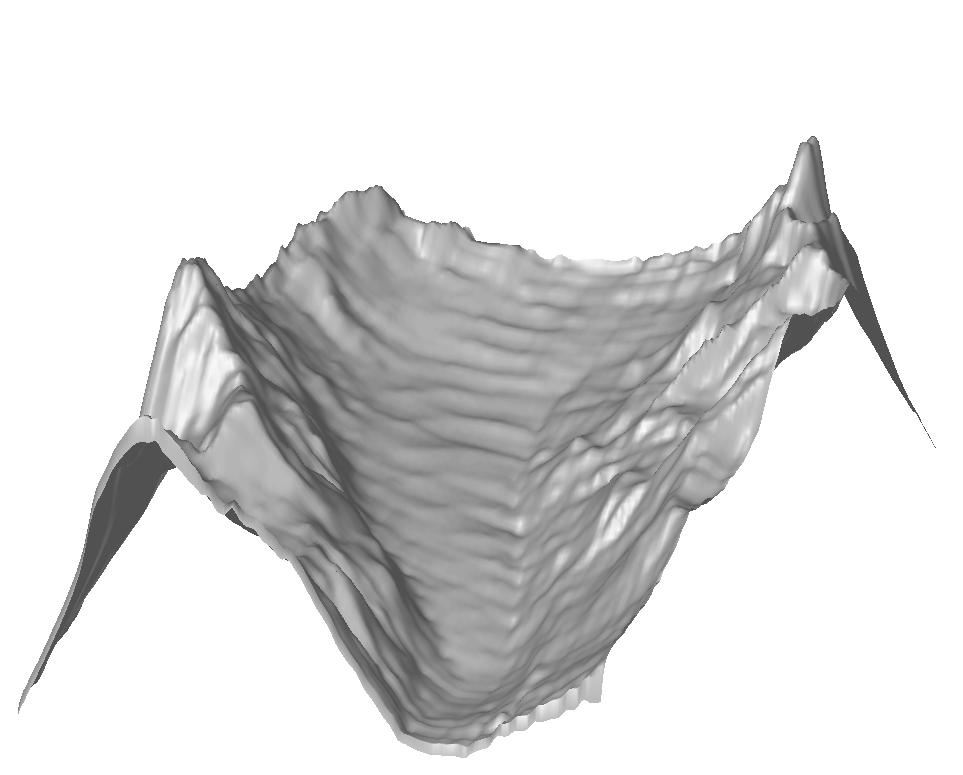
\includegraphics[width=6cm]{images/glacier1.eps} &
      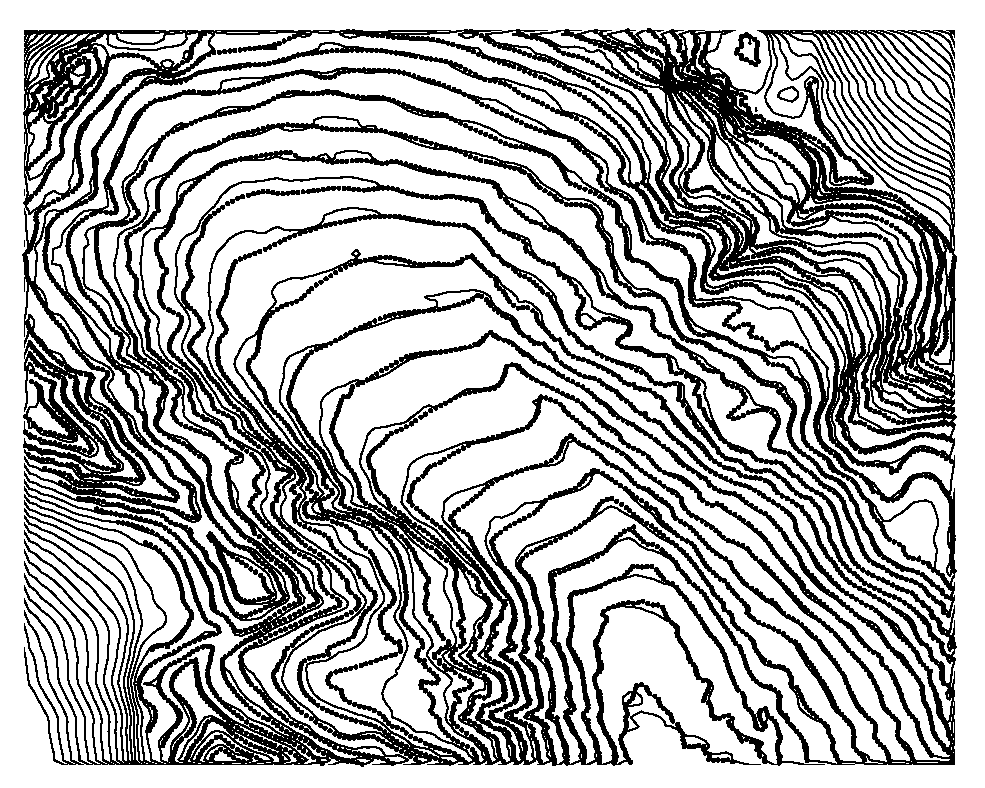
\includegraphics[width=6cm]{images/glacier2.eps}
    \end{tabular}
  \end{center}
  \caption{Reconstruction of the glacier data set {\tt vol87.dat} from
    \cite{Franke.Daten}, $M=8345$ nodes, $N=256$, $40$ iterations, tensor
    product damping factors $\hat w_{\zb k}$ to the weight function
    $g_{\frac{1}{2},3,10^{-3}}$; see {\tt glacier\/} in \cite{kupo02C}.
    Left: surface plot, Right: contour plot and sampling set
    ($\cdot$).\label{Fig:glacier}}
\end{figure}

%-----------------------------------------------------------------------------
\section{Conclusion}
%-----------------------------------------------------------------------------
We have shown that the optimal trigonometric interpolation problem at
$q$-separated nodes in $d$ dimensions is well conditioned for a polynomial
degree $N \ge 2d q^{-1}$.
In particular, an 'undersampling factor' less than $2$ suffices to ensure a
well conditioned univariate interpolation problem.
If we assume furthermore the uniformity condition $q=c M^{-\frac{1}{d}}$ for a
sampling set of cardinality $M$, then the total arithmetical complexity for
solving the interpolation problem \eqref{eq:optInterp} up to a prescribed
native error is of order ${\cal O}\left(M \log M \right)$.

{\bf Acknowledgement.}
The authors would like to thank J.~Prestin and G.~Steidl for numerous
fruitful and enlightening discussions.
The first author is grateful for partial support of this work by the German
Academic Exchange Service (DAAD) and the warm hospitality during his stay at
the Numerical Harmonic Analysis Group, University of Vienna.
%We would also like to thank the referees for their valuable
%suggestions.

\bibliographystyle{abbrv}
%\bibliography{/home/potts/tex/ref}
\bibliography{/home/kunis/Nfft3/nfft/trunk/doc/paper/references}
\end{document}
